\documentclass[letterpaper,10pt]{amsart}
\pagestyle{plain}


%%%%% Packages
\usepackage{soul}
\usepackage{graphicx,xcolor}
\usepackage{amsmath,amsthm}
\usepackage{amssymb}
\usepackage{float}
\usepackage{xcolor}
\usepackage{hyperref}
\hypersetup{colorlinks, linkcolor={red!50!black}, citecolor={green!50!black}, urlcolor={blue!50!black}}
%\usepackage[hidelinks]{hyperref}
\usepackage{enumerate}
\usepackage{mathrsfs}
\usepackage{mathtools}
\usepackage[english]{babel}



%%%%% Macros
\theoremstyle{plain}
\newtheorem*{theorem*}{Theorem}
\newtheorem{theorem}{Theorem}[section]
\newtheorem{theorems}[theorem]{Theorems}
\newtheorem{claim}{Claim}[section]
\newtheorem{definition}{Definition}[section]
\newtheorem{lemma}[theorem]{Lemma}
\newtheorem{proposition}[theorem]{Proposition}
\newtheorem{corollary}[theorem]{Corollary}
\newtheorem{conjecture}[theorem]{Conjecture}
\newtheorem*{question*}{Question}
\newtheorem*{questions*}{Questions}
\newtheorem*{remark*}{Remark}
\newtheorem*{example*}{Example}

\newcommand{\BS}[1][N]{\mathrm{BS}(1,#1)}
\def\htop{h_{\mathrm{top}}}


%%%%% Tikz
\usepackage{tikz}
\usetikzlibrary{patterns,positioning,arrows,decorations.markings,calc,decorations.pathmorphing,decorations.pathreplacing}
\usepackage{tikz-qtree}
\RequirePackage{pgffor} 


%%%%% Title and basic info
\title{Periodicity constraints and graph-coloring subshifts on solvable non-abelian Baumslag-Solitar groups}
\date{\today}
\author{Eduardo Silva}

\email{esilva@dim.uchile.cl}

\keywords{symbolic dynamics, groups, Baumslag-Solitar, subshifts of finite type, Cayley graphs, weak periodicity, frozen colorings, mixing properties, topological entropy}

%%%%% Start of document
\begin{document}
	


\begin{abstract}
For the Baumslag-Solitar group $\BS$, $N\ge 2$, we study how a synchronization between the geometry of the group and weak periodicity of a configuration in $\mathcal{A}^{\BS}$ forces global behavior in it, as well as in subshifts containing it. In particular we prove that a $\BS$-SFT which contains a configuration with period $a^{N^\ell}$, $\ell\ge 0$, must contain a strongly periodic configuration with monochromatic $a$-rows. Then we study proper $n$-colorings, $n\ge 3$, of the (right) Cayley graph of $\BS$, estimating the entropy of the associated subshift together with its mixing properties. We prove that $\BS$ admits a frozen $n$-coloring if and only if $n=3$.
\end{abstract}	
\maketitle 	

%%%%%%%%%%%%%%%%%%%%%%%%%%%%%%
%%%%%%%%%%%%%%%%%%%%%%%%%%%%%%


	\section{Introduction}
\label{section:introduction}
 The main object studied by symbolic dynamics on finitely generated groups are $\mathbf{G}$-\textbf{subshifts}, that is, closed subsets of the product space $\mathcal{A}^G$, for $\mathcal{A}$ a finite discrete alphabet and $G$ a finitely generated group, which are invariant under the action $\sigma$ of $G$ in $\mathcal{A}^G$, called the \textbf{shift} and defined by
  $$\sigma_g(x)_h=x_{g^{-1}h}\text{ for }x\in\mathcal{A}^G,\ g,h\in G.$$
An important family of subshifts are \textbf{subshifts of finite type (SFT)}, which are those that can be described completely by a finite set of forbidden patterns.

Throughout the last decades there has been interest in the cases $G=\mathbb{Z}^d$, $d\ge 2$, where a more complex structure arises in comparison with the one-dimensional case $G=\mathbb{Z}$: questions which have been long answered in the case $d=1$ become significantly more difficult for $d\ge 2$, sometimes changing its veracity, or remaining as open problems to this day. An example of this contrast is the so called Domino problem, which asks whether, given a finite set of forbidden patterns, the corresponding SFT is empty or not. For $d=1$ this problem is decidable, meanwhile for $d\ge 2$ it is undecidable.

In recent years interest has grown in studying symbolic dynamics on other finitely generated groups, obtaining results in a general context as well as in more particular settings, such as free groups or Baumslag-Solitar groups.

Given $m,n\in \mathbb{Z}\backslash \{0\}$, we define the corresponding \textbf{Baumslag-Solitar group} as given by its standard presentation
$$
\mathrm{BS}(m,n)\coloneqq \langle a,b \mid ba^mb^{-1}=a^n \rangle.
$$
These groups arise naturally as HNN-extensions of $\mathbb{Z}$, and were first introduced (though their origin might be older) in \cite{baumslag_solitar_1962} by G. Baumslag and D. Solitar, in order to provide an example of a non-Hopfian group with two generators and one relator, namely, one which is isomorphic to one of its (proper) quotient groups. Since then these groups have gained attention in the fields of combinatorial group theory and geometric group theory as examples and counterexamples of different properties (see \cite{harpe_2003,meskin_1972}), and more recently in the field of symbolic dynamics (see \cite{aubrun_kari_2013,cyr2016distortion,esnay2020weakly}).

The subfamily of Baumslag-Solitar groups $\BS$, $N\ge 2$, is of particular interest, since it exhibits nice properties in contrast with the rest of Baumslag-Solitar groups. This subfamily actually comprises all the cases for which the Baumslag-Solitar group is solvable, and hence amenable, while still being non-abelian (the case $N=1$ gives $\mathrm{BS}(1,1)\cong \mathbb{Z}^2$). In particular, this allows us to find a F\o lner sequence which permits us to define a notion of topological entropy for $\BS$-subshifts. 

In section \ref{section:preliminaries} we introduce the basic concepts and notation used throughout this work. We define the basic objects of symbolic dynamics, show how Baumslag-Solitar groups arise as HNN-extensions of $\mathbb{Z}$, explain the advantages of restricting ourselves to $\BS$, $N\ge 2$, and describe the structure of its Cayley graph, which allows us to state the following theorems in a geometric way.
	
	In section \ref{section:weak_periodicity} we show how the geometry of the group $\BS$ forces some rigidity for configurations in the full $\BS$-shift which exhibit weak periodicity in the direction of the generator $a$. Alternatively, how periods of powers of $N$ in the direction of $a$ force synchronization between $a$-rows of $\BS$. We show that a periodicity of $a^{pN^\ell}$, $\ell\ge 0$, $p\notin N\mathbb{Z}$ forces sufficiently high $a$-rows to be $p$-periodic (Theorem \ref{prop:bs_periodicity_p_generalcase}). Moreover, we show how having such a configuration affects a $\BS$-subshift which contains it (Theorem \ref{thm:subshift_with_configuration_rows_p_periodic_and_SFT}).

		\begin{theorem}\label{thm:summary_weak_periodicity}
			Let $x\in \mathcal{A}^{\BS}$, $\ell\ge 0$ and $p\notin N\mathbb{Z}$ be such that $a^{pN^{\ell}}\in \mathrm{Stab}(x)$. Then
			\begin{enumerate}
				\item all $a$-rows of level greater or equal than $\ell$ are $p$-periodic,
				\item if $X$ is a $\BS$-subshift which contains the configuration $x$, then there exists $y\in X$ for which all $a$-rows are $p$-periodic, and 
				\item if $X$ is further assumed to be an $SFT$ and $p=1$, then $y$ can be chosen to be strongly periodic.
			\end{enumerate}
		\end{theorem}

Given a group $G$ generated by a finite subset $S\subseteq G$ it is interesting to study the dynamical properties of proper colorings (in the sense used commonly in graph theory) of its Cayley graph. We define for $n\ge 2$ the \textbf{graph-coloring subshift} (GCS)
$$
\mathcal{C}_{n}\coloneqq\left\{x\in \{0,\ldots,n-1\}^G\mid \text{ for all } g\in G, s\in S: \ x_{g}\neq x_{gs} \right\},
$$
that is, each configuration $x\in \mathcal{C}_{n}$ describes a proper $n$-coloring of the Cayley graph $\Gamma(G,S)$ of $G$ with respect to the generator $S$. 
%The subshift $\mathcal{C}_{n}$ is always an SFT, since it can be described by the finite set of forbidden patterns 
%$$
%\mathcal{F}\coloneqq \left\{ \{x_{e_G}=i,x_{s}=i\}\mid i\in \{0,\ldots,n-1\}, s\in S \right\}.
%$$

Proper $n$-colorings of $G=\mathbb{Z}^2$, or more generally $G=\mathbb{Z}^d$ for $d\ge 2$, have been studied recently \cite{alon2019mixing, peled2018rigidity, ray2020proper}. In particular, in \cite{alon2019mixing} the authors study mixing properties for colorings of $\mathbb{Z}^d$, $d\ge 2$, introducing the notion of a frozen $n$-coloring of $\mathbb{Z}^d$ as an n-coloring which cannot be modified on a finite subset to create a different coloring, and prove that $\mathbb{Z}^d$ admits frozen $n$-colorings if and only if $2\le n\le d+1$. 


In section \ref{section:graph_coloring_subshifts} we consider the GCS $\mathcal{C}_n$ in $\BS$ and, among other results regarding extensibility of patterns and mixing properties, we show explicit constructions of frozen $3$-colorings in $\BS$ (Theorem \ref{thm:existence_frozen_3}), and then prove the lack of frozen $n$-colorings for every $n\ge 4$ (Theorem \ref{thm:no_frozen_n_ge_4}).

	\begin{theorem}\label{thm:summary_gcs_frozen_colorings}
		For $n\ge 3$, the GCS $\mathcal{C}_n\subseteq\{0,\ldots,n-1\}^{\BS}$ contains a frozen coloring if and only if $n=3$.
	\end{theorem}	

Another question of interest for $n$-colorings of a group $G$ is to estimate in how many different ways one can (properly) color a finite set, that is, the amount of patterns of $\mathcal{C}_n$ with a fixed (finite) support. The answer to this question, in turn, allows us to give estimates for the topological entropy of $\mathcal{C}_n$. This is a rather difficult question even when restricting the attention to $\mathbb{Z}^2$ and in general there are no closed formulas for any of these numbers, except for some exceptions as is the case of topological entropy of $3$-colorings of $\mathbb{Z}^2$, known to be $\frac{3}{2}\log\frac{4}{3}$ \cite{Lieb:1967zz}.


The last results of this paper provide bounds for the topological entropy of the GCS $\mathcal{C}_n$ in $\BS$ (Theorem \ref{thm:gcs_entropy_estimates}), as well as showing that the topological entropy of $\mathcal{C}_3$ is positive (Theorem \ref{thm:C_3_has_positive_entropy}).
	\begin{theorem} \label{thm:summary_gcs_entropy}
	For $n\ge 3$, the GCS $\mathcal{C}_n\subseteq\{0,\ldots,n-1\}^{\BS}$ satisfies
	
	$$
	\log(n-2)\le\htop(\mathcal{C}_n)\le\log(n-1).
	$$
	We also have that $\htop(\mathcal{C}_3)>0$. In fact, we further have that
	\begin{enumerate}
		\item if $N$ is odd then $\htop(\mathcal{C}_3)>\frac{1}{2}\log 2$, and
		\item if $N$ is even then $\htop(\mathcal{C}_3)>\frac{1}{2(2N+1)}\log 2$.
	\end{enumerate}
\end{theorem}
%%%%%%%%%%%%%%%%%%%%%%%%%%%%%%
%%%%%%%%%%%%%%%%%%%%%%%%%%%%%%


	\section{Preliminaries}\label{section:preliminaries}
	%A group $G$ is said to be \textbf{finitely generated} if it admits a group presentation $G=\langle S\mid R\rangle$, with $S$ finite. 
	
	\subsection{Symbolic dynamics on finitely generated groups}
	Let $G$ be a finitely generated group and $\mathcal{A}$ be a finite (discrete) set. Given $F\subseteq G$ finite, we call and element $p\in \mathcal{A}^{F}$ a \textbf{pattern}, $F$ its \textbf{support}, and use the notation $\mathrm{supp}(p)\coloneqq F$. Given patterns $p,q$, we say that $p$ is a subpattern of $q$, denoted $p\sqsubseteq q$, if there exists $g\in G$ such that $p=q|_{g\cdot \mathrm{supp}(p)}$. An element $x\in \mathcal{A}^G$ is called a \textbf{configuration} or \textbf{coloring}, and we use the notation $x_g\coloneqq x(g)$, $g\in G$. The set $\mathcal{A}^G$ can be endowed with the product topology, which is metrizable, compact and has a base given by the \textbf{cylinders}, that is, sets of the form
	$$
	[p]=\{x\in \mathcal{A}^G\mid x|_{\mathrm{supp}(p)}=p \}, \ p\text{ a pattern}.
	$$ 


	The topological space $\mathcal{A}^G$ together with the left $G$-action by homeomorphisms
	\begin{align*}
	\sigma:G&\to \mathrm{Homeo}(\mathcal{A}^G,\mathcal{A}^G)\\
	g&\mapsto \sigma_g,
	\end{align*}
	where for every $x\in \mathcal{A}^G$, $g,h\in G$:
	$$
	\sigma_g(x)_h=x_{g^{-1}h},
	$$
	is called the \textbf{full $G$-shift} and $\sigma$ is called the \textbf{shift} map. Associated to this action, we define for a configuration $x\in \mathcal{A}^G$ its \textbf{orbit} $$\mathrm{Orb}(x)\coloneqq\{\sigma_g(x)\mid g\in G \},$$ and its \textbf{stabilizer} $$\mathrm{Stab}(x)\coloneqq \{g\in G\mid \sigma_g(x)=x \}.$$ The latter of these sets is in fact a subgroup of $G$, and we have the relation $|\mathrm{Orb}(x)|=|G:\mathrm{Stab}(x)|$. A configuration $x\in \mathcal{A}^G$ is said to be \textbf{weakly periodic} if $\mathrm{Stab}(x)$ contains an infinite cyclic group, and \textbf{strongly periodic} if $|\mathrm{Orb}(x)|<\infty$.
	
	
	A subset $X\subseteq \mathcal{A}^G$ is called a \textbf{$G$-subshift} if it is closed and $\sigma$-invariant, that is, for every $g\in G$: $\sigma_g(X)=X$. Equivalently, $X$ is a \textbf{$G$-subshift} if there exists a family $\mathcal{F}$ of (forbidden) patterns such that
	$$
	X=\{x\in \mathcal{A}^G\mid \text{ for every }F\subseteq G \text{ finite: }x|_{F}\notin \mathcal{F}  \}.
	$$ 
	If such a family can be chosen finite we say that $X$ is a $G$-subshift of finite type (SFT).
	
	
	Given a $G$-subshift $X\subseteq \mathcal{A}^G$ described by a family $\mathcal{F}$ of (forbidden) patterns, we say that a pattern $p$ is \textbf{locally admissible} if $p$ does not contain elements of $\mathcal{F}$ a subpatterns, and \textbf{globally admissible} if there exists an $x\in X$ such that $x|_{\mathrm{supp}(p)}=p$.
	
	
	In the case where $G$ is amenable, we can define the \textbf{topological entropy} of a $G$-subshift $X$ as
	$$
	\htop(X)\coloneqq \lim_{n\to \infty}\frac{\log|\mathcal{L}_{F_n}(X)|}{|F_n|},
	$$
	where $\{F_n\}_{n\in \mathbb{N}}$ is a F\o lner sequence and $\mathcal{L}_{F_n}(X)=\{x|_{F_n}\mid x\in X\}$. This limit always exists and it does not depend on the F\o lner sequence chosen \cite[Theorem~4.38]{Kerr2016}. The topological entropy of a $G$-subshift $X$ represents the rate of exponential growth at which the amount of patterns with support $F_n$ we see in $X$ increases as these sets become more and more invariant.

%%%%%%%%%%%%%%%%%%%%%%%%%%%%%%

	  \subsection{HNN-extensions and Baumslag-Solitar groups}
Given a group $G$ and two isomorphic subgroups $H,K\le G$, the HNN-extension\footnote{The letters ``HNN'' stands for Higman, Neumann and Neumann, who introduced this kind of extension in \cite{HNN49}.} $G*_{\psi}$ is a group which contains a copy of $G$ in which $H$ and $K$ are conjugate subgroups.

\begin{definition}\label{definition.hnn_extension} Consider a group $G$ with a presentation $\langle S\left|\right. R\rangle$ and two isomorphic subgroups $H,K\le G$, with $\psi:K\to H$ an isomorphism. We define the \textbf{HNN-extension} of $G$ with respect to $\psi$ by the presentation
	$$
	G*_{\psi}\coloneqq \langle S\cup\{t\} \left|\right. R\cup \{t k t^{-1}=\psi(k): k\in K \} \rangle.
	$$
\end{definition}
Thanks to the relations of $G*_{\psi}$, for every $k\in K$ and $h\in H$ we have that $tk=\psi(k)t$ and $\psi^{-1}(h)t^{-1}=t^{-1}h$, which allows us to choose in which order the elements of $G$ appear with respect to $t$ or $t^{-1}$. By using this property, we can find a rather simple normal form for the HNN-extension $G*_{\psi}$, as the next proposition shows.

\begin{proposition}[{\cite[Theorem~IV.2.1]{lyndon_schupp_1977}}] \label{prop:hnn_general_normal_form}Let $G$ be a group, $H,K\le G$ and $\psi:K\to H$ an isomorphism. 
	Choose classes of representatives $T_H$ and $T_K$ of the right cosets for $H$ and $K$ in $G$, respectively, such that $T_H$ and $T_K$ both contain the identity element $e_G$. Then the HNN-extension $G*_\psi$ has a normal form given by the set of words of the form $g_0t^{\varepsilon_1}g_1t^{\varepsilon_2}\ldots t^{\varepsilon_n}g_n$ for $n\ge 0$, $g_0\in G$ and $\varepsilon_i\in \{+1,-1\}$ for $i=1,\ldots,n$, such that
	\begin{enumerate}
		\item $\varepsilon_i=1 $ implies $g_i\in T_K$,
		\item $\varepsilon_i=-1$ implies $g_i\in T_H$ and 
		\item there is no subword of the form $t^\varepsilon e_G t^{-\varepsilon}$, for $\varepsilon\in\{+1,-1\}$.
	\end{enumerate} 
\end{proposition}

An important example of HNN-extensions are \textbf{Baumslag-Solitar groups}, to which we turn our attention now. Given $m,n\in \mathbb{Z}\backslash\{0\}$ we define the group 
$$\mathrm{BS}(m,n)=\langle a,b \left|\right. ba^mb^{-1}=a^n\rangle,$$ 

which is an HNN-extension of $\mathbb{Z}$ via the isomorphism $\psi:\langle a^m \rangle\to \langle a^n\rangle$ which maps $\psi(a^m)=a^n$.

Throughout the rest of this work we center our attention on the groups $\mathrm{BS}(1,N)$ for $N\ge 2$, which cover (up to isomorphisms) the solvable non-abelian case. Restricting ourselves to this subfamily has many advantages: we have useful commuting relations between the elements of the group, a simpler normal form (in contrast to the general one for HNN-extensions) and a better understanding of the structure of the Cayley graph of the group, all of which we describe in further detail below.

First we establish the following lemma, which summarizes some of the consequences induced by the defining relation used in the standard presentation of $\BS$. Its elementary proof is by induction and is omitted. These additional relations will prove useful in arriving at a normal form for $\BS$ below.

\begin{lemma}\label{prop:bs_further_identifications} The unique relation $bab^{-1}=a^N$ used to define $\BS$ forces further identifications: for every $j\ge 0$ and $k\in \mathbb{Z}$ we have $b^{j}a^k=a^{kN^j}b^j$.
\end{lemma}

\begin{proposition}\label{prop:normalform_bsgroups}
	The solvable non-abelian Baumslag-Solitar groups $\BS$, $N\ge 2$, have a normal form given by words $b^{-j}a^kb^{i}$ where $i,j\ge 0$ and $k\in \mathbb{Z}$, and $k\in N\mathbb{Z}$ only if $i=0$ or $j=0$.
\end{proposition}

\begin{proof}
	Using the normal form for HNN-extensions described in Proposition \ref{prop:hnn_general_normal_form} with sets of representatives $T_K=\{e_{\BS}\}$ and $T_H=\{e_{\BS},a,\ldots,a^{N-1}\}$, we distinguish three types of words.
	
	\begin{enumerate}[1.]
		\item The first type are words of the form $a^kb^i$, for $k\in\mathbb{Z} $, $i\ge 0$. This word is already in the form described in the proposition so in this case we are finished.
		\item The second type are words of the form $a^{k_0}b^{-1}a^{k_1}\cdots b^{-1}a^{k_n}$, for $k_0\in \mathbb{Z}$, and $0\le k_1,\ldots,k_n<N$. We will prove we can arrive at the normal form described in the proposition by induction. Moreover, we will prove that there exists $k'\in \mathbb{Z}$ such that $a^{k_0}b^{-1}a^{k_1}\cdots b^{-1}a^{k_n}=b^{-n}a^{Nk'}a^{k_n}$. 
		
		If $n=1$, then we can use the relation from the HNN-extension to obtain
		$$
		a^{k_0}b^{-1}a^{k_1}=b^{-1}a^{Nk_0}a^{k_1}.
		$$
		In the general case for $n\ge 2$, by the induction hypothesis we know that for some $k'\in \mathbb{Z}$ we have $$a^{k_0}b^{-1}a^{k_1}\cdots b^{-1}a^{k_{n-1}}=b^{-(n-1)}a^{Nk'}a^{k_{n-1}}.$$
		
		Then
		\begin{align*}
	a^{k_0}b^{-1}a^{k_1}\cdots b^{-1}a^{k_{n-1}}b^{-1}a^{k_n}&=b^{-(n-1)}a^{Nk'}a^{k_{n-1}}b^{-1}a^{k_n}\\
		&=b^{-n}a^{N(Nk'+k_{n-1})}a^{k_n},
		\end{align*}
		finishing the induction.
		\item Finally, the third type are words of the form $a^{k_0}b^{-1}a^{k_1}\cdots b^{-1}a^{k_n}b^{j}$, for $k_0\in \mathbb{Z}$, $0\le k_1,\ldots,k_n<N$ and $j\ge 1$. Proceeding as in the previous case, we show that there must exist $k'\in \mathbb{Z}$ such that
		$$
		a^{k_0}b^{-1}a^{k_1}\cdots b^{-1}a^{k_n}b^{j}=b^{-n}a^{Nk'}a^{k_n}b^{j}
		$$
		
		Note that as $j\ge 1$, the third condition from Proposition \ref{prop:hnn_general_normal_form} ensures that $k_n\neq 0$ (since otherwise the considered word would contain a subword of the form $b^{-1}e_{\BS}b$, which is forbidden), and hence the exponent $Nk'+k_n$ of $a$ is not a number in $N\mathbb{Z}$.
	\end{enumerate}
\end{proof}
In Baumslag-Solitar groups, being solvable is equivalent to being amenable, so when restricting ourselves to $\BS$ we are also covering the amenable Baumslag-Solitar groups. It is actually possible to exhibit an explicit (right) F\o lner sequence, which proves itself to be useful for computing topological entropy, as well as for making constructions in the group.

\begin{proposition}\label{prop:rectangles_and_folner} For $N\ge 2$ and $m\ge 1$, define the \textbf{rectangle of height $m$}
	$$
	R_m\coloneqq \{a^kb^i\mid 0\le k<N^m, \ 0\le i<m  \}\subseteq \BS.
	$$
	Then $\{R_m\}_{m\ge 1}$ forms a F\o lner sequence in $\BS$.
\end{proposition}




%%%%%%%%%%%%%%%%%%%%%%%%%%%%%%

\subsection{The Cayley graph of $\BS$}
To finish this section let us take a look at the structure of the Cayley graph of $\BS$. Recall that given a group $G$ together with a finite generating set $S\subseteq G$, the \textbf{(right) Cayley graph} of $G$ with respect to $S$ is the labeled directed graph  $\Gamma(G,S)=(V_{\Gamma},E_{\Gamma},\lambda_{\Gamma})$ where
\begin{enumerate}
	\item the set of vertices is $V_\Gamma=G$, 
	\item the set of edges is $E_{\Gamma}=\{(g,gs)\in G\times G\mid s\in S\}$, and
	\item the labeling function $\lambda_{\Gamma}:E_{\Gamma}\to V_{\Gamma}$ satisfies $\lambda_{\Gamma}(g,gs)=s$, for $g\in G$, $s\in S$.
\end{enumerate}


A section of the Cayley graph of $\BS$ with respect to the generating set $S=\{a,b\}$ is shown in Figure \ref{fig:section_cayley_graph_bs}, where we see that its structure is that of rows (along the edges labeled by the $a$-generator) being arranged (in a sideways view) as an N-ary tree. Seen from the front, each row has below it (i.e.\ in the $b^{-1}$-direction) a unique $a$-row, and above it (i.e.\ in the $b$-direction) $N$ new $a$-rows. More formally, defining $A\coloneqq\{a^k \mid k\in\mathbb{Z}\}$, a set of the form $gA$ for $g\in \BS$ will be called an $\mathbf{a}$\textbf{-row} of the Cayley graph of $\BS$, meanwhile a set of the form $\displaystyle\bigcup_{n=1}^{\infty}gb^{-n}A  \cup\bigcup_{n=0}^\infty\left( g\prod_{s=1}^{n}(a^{i_s}b)A \right)$ for $g\in \BS$ and a sequence $\{i_s\}_{s=1}^{\infty}\in \{0,\ldots,N-1\}^{\mathbb{N}}$ will be called a \textbf{sheet} of the Cayley graph of $\BS$. An example of the latter is illustrated in Figure \ref{fig:bssheet}. 

In the drawings of the Cayley graph of $\BS$ made in the next sections we will omit the label as well as the direction of the edges from the drawing, as they are not relevant for the context they are used in.

We finish this section by making the following definition, which enables us to enunciate the results of the next section in a clearer way.
\begin{definition}For $g\in \BS$ we define the \textbf{$a$-row containing $g$} as 
	$$
	\Gamma_g\coloneqq\{ ga^k\mid k\in \mathbb{Z}\}.
	$$
	Using the normal form to write $g=b^{-j}a^kb^i$, for $i,j\ge 0$ and $k\in \mathbb{Z}$ such that $k\in N\mathbb{Z}$ is only possible if $i=0$ or $j=0$, we say that $\Gamma_g$ is an \textbf{$a$-row at level } $i-j$. Note that since the normal form of an element is unique, the level of the corresponding $a$-row $\Gamma_g$ is well defined.
\end{definition}
\begin{figure}[h]
	\centering
	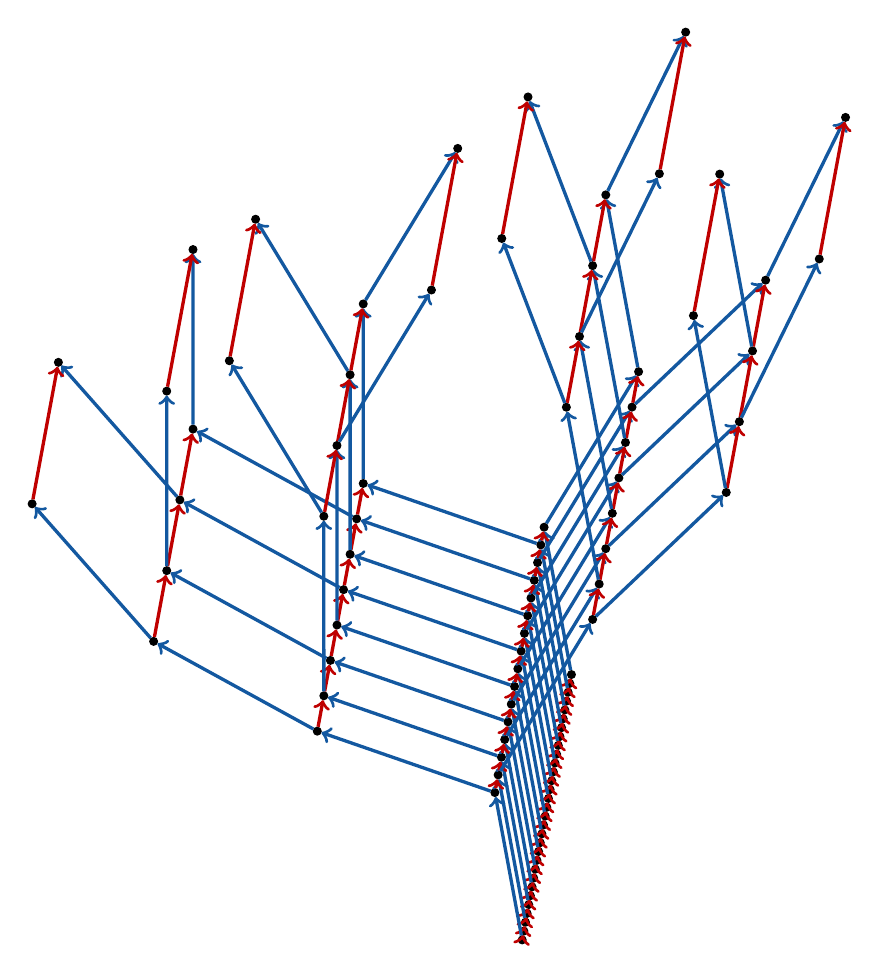
\begin{tikzpicture}
	[xscale=0.4,yscale=0.38,node distance=0.5cm,
	nn/.style={circle,fill,draw=black,inner sep=1pt},font=\small]
	%%%%% LEVEL -1
	\node[nn] (nivelm10) at (0,0) {};
	\foreach \i[remember=\i as \lasti (initially 0)] in {1,...,30}
	{
	\node[nn] (nivelm1\i) at ([shift=({80:0.3 cm})]nivelm1\lasti) {};
	\path[->, very thick,draw={rgb, 255:red, 191; green, 0; blue, 0 }] (nivelm1\lasti) edge (nivelm1\i);
	};
	%%%%% LEVEL 0
	\foreach \i[remember=\i as \lasti (initially 0)] in {0,2,...,30}
	{
	\node[nn] (nivel0\i) at ([shift=({100:5 cm})]nivelm1\i) {};
	\path[->, very thick,draw={rgb, 255:red, 19; green, 88; blue, 160 }] (nivelm1\i) edge (nivel0\i);
	\ifnum \i>0
	\path[->, very thick,draw={rgb, 255:red, 191; green, 0; blue, 0 }] (nivel0\lasti) edge (nivel0\i);
	\fi 
	};
	%%%%% LEVEL 1
	\foreach \i[remember=\i as \lasti (initially 0)] in {0,4,...,30}
	{
	\node[nn] (nivel1\i) at ([shift=({160:6 cm})]nivel0\i) {};
	\path[->, very thick,draw={rgb, 255:red, 19; green, 88; blue, 160 }] (nivel0\i) edge (nivel1\i);
	\ifnum \i>0
	\path[->, very thick,draw={rgb, 255:red, 191; green, 0; blue, 0 }] (nivel1\lasti) edge (nivel1\i);
	\fi 
	};
	\foreach \i[remember=\i as \lasti (initially 2)] in {2,6,...,30}
{
	\node[nn] (nivel1\i) at ([shift=({60:6 cm})]nivel0\i) {};
	\path[->, very thick,draw={rgb, 255:red, 19; green, 88; blue, 160 }] (nivel0\i) edge (nivel1\i);
	\ifnum \i>2
	\path[->, very thick,draw={rgb, 255:red, 191; green, 0; blue, 0 }] (nivel1\lasti) edge (nivel1\i);
	\fi 
};
    %%%%% LEVEL 2
    \foreach \i[remember=\i as \lasti (initially 0)] in {0,8,...,30}
    {
    	\node[nn] (nivel2\i) at ([shift=({150:6 cm})]nivel1\i) {};
    	\path[->, very thick,draw={rgb, 255:red, 19; green, 88; blue, 160 }] (nivel1\i) edge (nivel2\i);
    	\ifnum \i>0
    	\path[->, very thick,draw={rgb, 255:red, 191; green, 0; blue, 0 }] (nivel2\lasti) edge (nivel2\i);
    	\fi 
    };
    \foreach \i[remember=\i as \lasti (initially 4)] in {4,12,...,30}
{
	\node[nn] (nivel2\i) at ([shift=({90:6 cm})]nivel1\i) {};
	\path[->, very thick,draw={rgb, 255:red, 19; green, 88; blue, 160 }] (nivel1\i) edge (nivel2\i);
	\ifnum \i>4
	\path[->, very thick,draw={rgb, 255:red, 191; green, 0; blue, 0 }] (nivel2\lasti) edge (nivel2\i);
	\fi 
};
    \foreach \i[remember=\i as \lasti (initially 2)] in {2,10,...,30}
{
	\node[nn] (nivel2\i) at ([shift=({45:6 cm})]nivel1\i) {};
	\path[->, very thick,draw={rgb, 255:red, 19; green, 88; blue, 160 }] (nivel1\i) edge (nivel2\i);
	\ifnum \i>2
	\path[->, very thick,draw={rgb, 255:red, 191; green, 0; blue, 0 }] (nivel2\lasti) edge (nivel2\i);
	\fi 
};
    \foreach \i[remember=\i as \lasti (initially 6)] in {6,14,...,30}
{
	\node[nn] (nivel2\i) at ([shift=({100:6 cm})]nivel1\i) {};
	\path[->, very thick,draw={rgb, 255:red, 19; green, 88; blue, 160 }] (nivel1\i) edge (nivel2\i);
	\ifnum \i>6
	\path[->, very thick,draw={rgb, 255:red, 191; green, 0; blue, 0 }] (nivel2\lasti) edge (nivel2\i);
	\fi 
};
	%%%% LEVEL 3
 \foreach \i[remember=\i as \lasti (initially 0)] in {0,16,...,30}
{
	\node[nn] (nivel3\i) at ([shift=({130:6 cm})]nivel2\i) {};
	\path[->, very thick,draw={rgb, 255:red, 19; green, 88; blue, 160 }] (nivel2\i) edge (nivel3\i);
	\ifnum \i>0
	\path[->, very thick,draw={rgb, 255:red, 191; green, 0; blue, 0 }] (nivel3\lasti) edge (nivel3\i);
	\fi 
};
 \foreach \i[remember=\i as \lasti (initially 2)] in {2,18,...,30}
{
	\node[nn] (nivel3\i) at ([shift=({100:6 cm})]nivel2\i) {};
	\path[->, very thick,draw={rgb, 255:red, 19; green, 88; blue, 160 }] (nivel2\i) edge (nivel3\i);
	\ifnum \i>2
	\path[->, very thick,draw={rgb, 255:red, 191; green, 0; blue, 0 }] (nivel3\lasti) edge (nivel3\i);
	\fi 
};
 \foreach \i[remember=\i as \lasti (initially 4)] in {4,20,...,30}
{
	\node[nn] (nivel3\i) at ([shift=({120:6 cm})]nivel2\i) {};
	\path[->, very thick,draw={rgb, 255:red, 19; green, 88; blue, 160 }] (nivel2\i) edge (nivel3\i);
	\ifnum \i>4
	\path[->, very thick,draw={rgb, 255:red, 191; green, 0; blue, 0 }] (nivel3\lasti) edge (nivel3\i);
	\fi 
};
 \foreach \i[remember=\i as \lasti (initially 6)] in {6,22,...,30}
{
	\node[nn] (nivel3\i) at ([shift=({110:6 cm})]nivel2\i) {};
	\path[->, very thick,draw={rgb, 255:red, 19; green, 88; blue, 160 }] (nivel2\i) edge (nivel3\i);
	\ifnum \i>6
	\path[->, very thick,draw={rgb, 255:red, 191; green, 0; blue, 0 }] (nivel3\lasti) edge (nivel3\i);
	\fi 
};
 \foreach \i[remember=\i as \lasti (initially 8)] in {8,24,...,30}
{
	\node[nn] (nivel3\i) at ([shift=({90:6 cm})]nivel2\i) {};
	\path[->, very thick,draw={rgb, 255:red, 19; green, 88; blue, 160 }] (nivel2\i) edge (nivel3\i);
	\ifnum \i>8
	\path[->, very thick,draw={rgb, 255:red, 191; green, 0; blue, 0 }] (nivel3\lasti) edge (nivel3\i);
	\fi 
};
 \foreach \i[remember=\i as \lasti (initially 10)] in {10,26,...,30}
{
	\node[nn] (nivel3\i) at ([shift=({65:6 cm})]nivel2\i) {};
	\path[->, very thick,draw={rgb, 255:red, 19; green, 88; blue, 160 }] (nivel2\i) edge (nivel3\i);
	\ifnum \i>10
	\path[->, very thick,draw={rgb, 255:red, 191; green, 0; blue, 0 }] (nivel3\lasti) edge (nivel3\i);
	\fi 
};
 \foreach \i[remember=\i as \lasti (initially 12)] in {12,28,...,30}
{
	\node[nn] (nivel3\i) at ([shift=({60:6 cm})]nivel2\i) {};
	\path[->, very thick,draw={rgb, 255:red, 19; green, 88; blue, 160 }] (nivel2\i) edge (nivel3\i);
	\ifnum \i>12
	\path[->, very thick,draw={rgb, 255:red, 191; green, 0; blue, 0 }] (nivel3\lasti) edge (nivel3\i);
	\fi 
};
 \foreach \i[remember=\i as \lasti (initially 14)] in {14,30}
{
	\node[nn] (nivel3\i) at ([shift=({65:6 cm})]nivel2\i) {};
	\path[->, very thick,draw={rgb, 255:red, 19; green, 88; blue, 160 }] (nivel2\i) edge (nivel3\i);
	\ifnum \i>14
	\path[->, very thick,draw={rgb, 255:red, 191; green, 0; blue, 0 }] (nivel3\lasti) edge (nivel3\i);
	\fi 
};
	\end{tikzpicture}
	\caption{A section of the Cayley graph of $BS(1,2)$.  Red edges are labeled with ``$a$'', while blue edges are labeled with ``$b$''.}
	\label{fig:section_cayley_graph_bs}
\end{figure}
\begin{figure}[H]
	\centering
	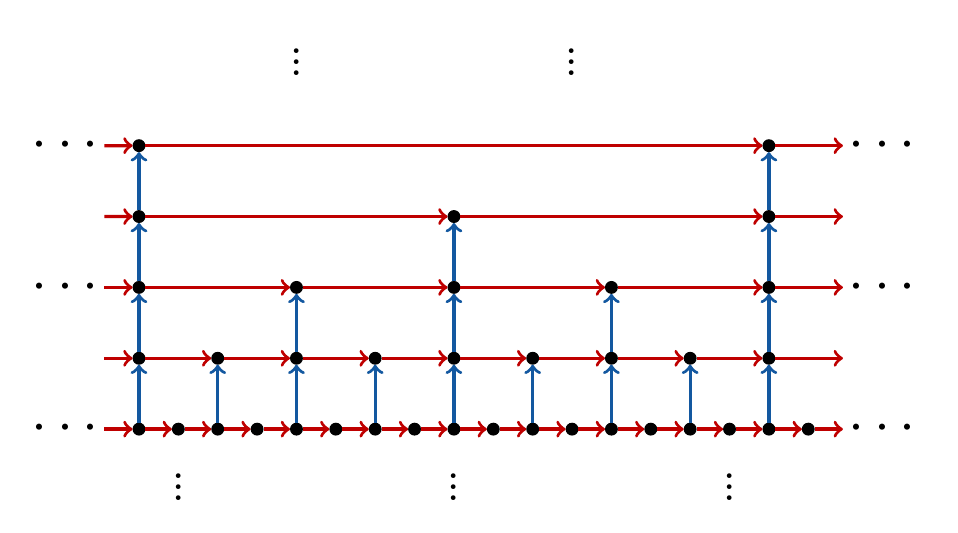
\begin{tikzpicture}
	[yscale=0.9,xscale=0.25,
	nn/.style={circle,fill,draw=black,inner sep=1.8pt},font=\small]
	\begin{scope}[auto, every node/.style={inner sep=1.5pt}]
	%LEVEL 0
	\node[font=\fontsize{20}{20}\selectfont] (leftdots) at (8,5.3) {$\vdots$};
	\node[font=\fontsize{20}{20}\selectfont] (leftdots) at (22,5.3) {$\vdots$};
	\node[font=\fontsize{20}{20}\selectfont] (leftdots) at (-3.5,0) {$\cdots$};
	\node[font=\fontsize{20}{20}\selectfont] (leftdots2) at (-3.5,4) {$\cdots$};
	\node[font=\fontsize{20}{20}\selectfont] (leftdots2) at (-3.5,2) {$\cdots$};
	\node[font=\fontsize{20}{20}\selectfont] (rightdots) at (38,0) {$\cdots$};	
	\node[font=\fontsize{20}{20}\selectfont] (rightdots) at (38,2) {$\cdots$};	
	\node[font=\fontsize{20}{20}\selectfont] (rightdots2) at (38,4) {$\cdots$};		
	\node[font=\fontsize{20}{20}\selectfont] (rightdots2) at (2,-0.7) {$\vdots$};	
	\node[font=\fontsize{20}{20}\selectfont] (rightdots2) at (16,-0.7) {$\vdots$};				
	\node[font=\fontsize{20}{20}\selectfont] (rightdots2) at (30,-0.7) {$\vdots$};							
	\foreach \x in {0,...,3}
	\node[shape=circle,draw=black,fill] (a\x) at (2*\x,0) {};
	\foreach \x in {4,...,7}
	\node[shape=circle,draw=black,fill] (a\x) at (2*\x,0) {};	
	\foreach \x in {8,...,11}
	\node[shape=circle,draw=black,fill] (a\x) at (2*\x,0) {};
	\foreach \x in {12,...,15}
	\node[shape=circle,draw=black,fill] (a\x) at (2*\x,0) {};			
	\foreach \x in {16,...,17}
	\node[shape=circle,draw=black,fill] (a\x) at (2*\x,0) {};
	\foreach \x in {0,...,16}
	\pgfmathtruncatemacro{\j}{\x+1}
	\path[->, very thick,draw={rgb, 255:red, 191; green, 0; blue, 0 }](a\x) edge node[below] {} (a\j);
	%LEVEL 1
	\foreach \x in {0,2,8,10,16}
	{
		\node[shape=circle,draw=black,fill] (a\x b) at (2*\x,1) {};
		\path[->,very thick,draw={rgb, 255:red, 19; green, 88; blue, 160 }](a\x) edge node[left] {} (a\x b);
	};
	\foreach \x in {4,6,12,14}
	{
		\node[shape=circle,draw=black,fill] (a\x b) at (2*\x,1) {};
		\path[->, very thick, draw={rgb, 255:red, 19; green, 88; blue, 160 }](a\x) edge node[left] {} (a\x b);
	};
	\foreach \x in {0,2,4,6,8,10,12,14}
	{
		\pgfmathtruncatemacro{\j}{\x+2}
		\path[->, very thick, draw = {rgb, 255:red, 191; green, 0; blue, 0 }](a\x b) edge node[below] {} (a\j b);
	};
	%LEVEL 2
	\foreach \x in {0,4,8,12,16}
	{
		\node[shape=circle,draw=black,fill] (a\x b2) at (2*\x,2) {};
		\path[->, very thick, draw={rgb, 255:red, 19; green, 88; blue, 160 }](a\x b) edge node[left] {} (a\x b2);
	};
	\foreach \x in {0,4,8,12}
	{
		\pgfmathtruncatemacro{\j}{\x+4}
		\path[->, very thick, draw={rgb, 255:red, 191; green, 0; blue, 0 }](a\x b2) edge node[below] {} (a\j b2);
	};
	%LEVEL 3
	\foreach \x in {0,8,16}
	{
		\node[shape=circle,draw=black,fill] (a\x b3) at (2*\x,3) {};
		\path[->, very thick, draw={rgb, 255:red, 19; green, 88; blue, 160 }](a\x b2) edge node[left] {} (a\x b3);
	};
	\foreach \x in {0,8}
	{
		\pgfmathtruncatemacro{\j}{\x+8}
		\path[->,very thick, draw={rgb, 255:red, 191; green, 0; blue, 0 }](a\x b3) edge node[below] {} (a\j b3);
	};
	%LEVEL 4
	\foreach \x in {0,16}
	{
		\node[shape=circle,draw=black,fill] (a\x b4) at (2*\x,4) {};
		\path[->, very thick, draw={rgb, 255:red, 19; green, 88; blue, 160 }](a\x b3) edge node[left] {} (a\x b4);
	};
	\path[->, very thick, draw={rgb, 255:red, 191; green, 0; blue, 0 }](a0b4) edge node[below] {} (a16b4);
	\node[] (f0) at (36,0) {};
	\path[->,very thick, draw={rgb, 255:red, 191; green, 0; blue, 0 }](a17) edge node[below] {} (f0);
	\node[] (f1) at (36,1) {};
	\path[->,very thick, draw={rgb, 255:red, 191; green, 0; blue, 0 }](a16b) edge node[below] {} (f1);
	\node[] (f2) at (36,2) {};
	\path[->,very thick, draw={rgb, 255:red, 191; green, 0; blue, 0 }](a16b2) edge node[left] {} (f2);
	\node[] (f3) at (36,3) {};
	\path[->,very thick, draw={rgb, 255:red, 191; green, 0; blue, 0 }](a16b3) edge node[below] {} (f3);
	\node[] (f4) at (36,4) {};
	\path[->,very thick, draw={rgb, 255:red, 191; green, 0; blue, 0 }](a16b4) edge node[below] {} (f4);
	
	\node[] (i0) at (-2,0) {};
	\path[<-,very thick, draw={rgb, 255:red, 191; green, 0; blue, 0 }](a0) edge node[left] {} (i0);
	\node[] (i1) at (-2,1) {};
	\path[<-,very thick, draw={rgb, 255:red, 191; green, 0; blue, 0 }](a0b) edge node[left] {} (i1);
	\node[] (i2) at (-2,2) {};
	\path[<-,very thick, draw={rgb, 255:red, 191; green, 0; blue, 0 }](a0b2) edge node[left] {} (i2);
	\node[] (i3) at (-2,3) {};
	\path[<-,very thick, draw={rgb, 255:red, 191; green, 0; blue, 0 }](a0b3) edge node[left] {} (i3);
	\node[] (i4) at (-2,4) {};
	\path[<-,very thick, draw={rgb, 255:red, 191; green, 0; blue, 0 }](a0b4) edge node[left] {} (i4);
	\end{scope}	
	\end{tikzpicture}
	\caption{A section of a sheet of the Cayley graph of $BS(1,2)$.  Red edges are labeled with ``$a$'', while blue edges are labeled with ``$b$''.}
	\label{fig:bssheet}
\end{figure}

%%%%%%%%%%%%%%%%%%%%%%%%%%%%%%
%%%%%%%%%%%%%%%%%%%%%%%%%%%%%%
	
	
	\section{Periodicity constraints}\label{section:weak_periodicity}

	This section focuses on studying how (weakly) periodic configurations on $\mathcal{A}^{\BS}$ exhibit some rigidity when their stabilizer and the structure of the Cayley graph of the group synchronize in some sense. In particular, we will study weak periodicity in the $a$-direction and obtain results regarding the structure of $a$-rows of configurations with this periodicity.
	
	\begin{proposition}\label{prop:bs_periodicity_p_generalcase}
		Let $x\in \mathcal{A}^{\BS}$, $\ell\ge 0$ and $p\notin N\mathbb{Z}$ be such that $a^{pN^\ell}\in \mathrm{Stab}(x)$. Then every $a$-row of level greater or equal than $\ell$ is $p$-periodic. That is, for every $i,j\ge 0$, $k,m\in \mathbb{Z}$:
		$$
		x_{b^{-j}a^kb^{j+i+\ell}a^{m+p}}=x_{b^{-j}a^kb^{j+i+\ell}a^{m}}.
		$$
		Moreover, if we further assume that $\gcd(p,N)=1$, then for every $i\ge \ell$ and $h\ge 0$ all the $a$-rows of level $i+h$ sharing a common base $a$-row of level $i$ are equal, up to a translation. More precisely, for every $h\ge 0$ there exists $r\in \mathbb{Z}$ such that for every $j\ge 0$, $i\ge \ell$, $k,m\in \mathbb{Z}$ and $q\in \{0,\ldots,N^h-1\}$:
		$$
		x_{b^{-j}a^{k}b^{j+i+h}a^{m}}=x_{b^{-j}a^{k}b^{j+i}a^{q}b^{h}a^{m-qr}}.
		$$
		
	\end{proposition}
	\begin{proof}
		By the hypothesis we have that $x$ is $a^{pN^\ell}$ periodic: 
		$$\sigma_{a^{pN^\ell}}(x)=x.$$
		Note that for $i,j\ge 0$ and $k,m\in \mathbb{Z}$ we can use the commuting relations from Proposition \ref{prop:bs_further_identifications} and show that
		\begin{align*}
		b^{-j}a^kb^{j+i+\ell}a^{m+p}&=b^{-j}a^ka^{pN^{j+i+\ell}}b^{j+i+\ell}a^{m}\\
		&=b^{-j}a^{pN^{i+\ell}N^j}a^{k}b^{j+i+\ell}a^{m}\\
		&=a^{pN^{i+\ell}}b^{-j}a^{k}b^{j+i+\ell}a^{m}\\
		&=a^{N^{i}pN^{\ell}}b^{-j}a^{k}b^{j+i+\ell}a^{m}.
		\end{align*}
		As $\sigma_{a^{pN^{\ell}}}(x)=x$ we also have that $\sigma_{a^{N^{i}pN^{\ell}}}(x)=x$. Hence
		\begin{align*}
		x_{b^{-j}a^kb^{j+i+\ell}a^{m+p}}&=x_{a^{N^{i}pN^{\ell}}b^{-j}a^{k}b^{j+i+\ell}a^{m}}\\
		&=x_{b^{-j}a^{k}b^{j+i+\ell}a^{m}}.
		\end{align*}
		This proves that every $a$-row of level greater or equal than $\ell$ is $p$-periodic, seen as a bi-infinite sequence.
		
		
		For the second part of the proposition, note that as we assume that $\gcd(p,N)=1$ then for every $h\ge 1$ we have $\gcd(p,N^h)=1$. Hence by Bézout's identity there must exist $r,s\in \mathbb{Z}$ such that $1=sp+rN^h$. 
		
		
		Using the above and again the identities from Proposition \ref{prop:bs_further_identifications}, we see that for $j\ge 0$, $i\ge \ell$, $k,m\in \mathbb{Z}$ and $q\in \{0,\ldots,N^h-1\}$:
		\begin{align*}
		b^{-j}a^{k}b^{j+i}a^{q}b^{h}a^{m-qr}&==b^{-j}a^{k}b^{j+i}a^{q-qrN^h}b^{h}a^{m}\\
		&=b^{-j}a^{k}a^{q(1-rN^{h})N^{i+j}}b^{j+i}b^{h}a^{m}\\
		&=b^{-j}a^{q(1-rN^{h})N^{i}N^{j}}a^{k}b^{j+i}b^{h}a^{m}\\	
		&=a^{q(1-rN^{h})N^{i}}b^{-j}a^{k}b^{j+i}b^{h}a^{m}\\
		&=a^{qspN^{i-\ell}N^{\ell}}b^{-j}a^{k}b^{j+i}b^{h}a^{m}\\
		&=a^{qsN^{i-\ell}pN^{\ell}}b^{-j}a^{k}b^{j+i}b^{h}a^{m}.				
		\end{align*}
		Then as $\sigma_{a^{pN^\ell}}(x)=x$ we also have that $\sigma_{a^{qsN^{i-\ell}pN^{\ell}}}(x)=x$ and hence
		\begin{align*}
		x_{b^{-j}a^{k}b^{j+i}a^{q}b^{h}a^{m-qr}}&=x_{a^{qsN^{i-\ell}pN^{\ell}}b^{-j}a^{k}b^{j+i}b^{h}a^{m}}\\
		&=x_{b^{-j}a^{k}b^{j+i}b^{h}a^{m}}.
		\end{align*}
		The above proves that, for $q\in \{0,\ldots,N^h-1\}$, all $a$-rows $\Gamma_{b^{-j}a^kb^{j+i}a^qb^h}$ at level $i+h$ originating from the $a$-row $\Gamma_{b^{-j}a^kb^{j+i}}$ have the same sequence in $x$, namely $\{x_{b^{-j}a^{k}b^{j+i}b^{h}a^{m}}\}_{m\in \mathbb{Z}}$, up to a translation of $qr$.
	\end{proof}
	
	\begin{remark*} The second part of the previous propositon still holds if one does not assume that $\gcd(p,N)=1$, with the slight alteration of requiring $i\ge \ell+1$ instead of $i\ge \ell$. To prove this it is sufficient to note that $\sigma_{a^{pN^\ell}}(x)=x$ and $d\coloneqq \gcd(p,N)$, then we also have $\sigma_{a^{\frac{N}{d}pN^\ell}}(x)=x$ and hence 
		$$
		\sigma_{a^{\frac{p}{d}N^{\ell+1}}}(x)=x,
		$$
		from which we can apply Proposition \ref{prop:bs_periodicity_p_generalcase}.
	\end{remark*}
	
	\begin{corollary} Let $x\in \mathcal{A}^{\BS}$ be a strongly periodic configuration such that there exists $\ell\ge 0$ with $a^{pN^{\ell}}\in \mathrm{Stab}(x).$ Then for every $g\in \BS$ the $a$-row $\Gamma_g$ containing $g$ in $x$ has period $p$. That is, for every $m\in \mathbb{Z}$:
		$$
		x_{ga^{m}}=x_{ga^{m+p}}.
		$$
	\end{corollary}
	\begin{proof}
		Since $x$ is strongly periodic, it has a finite orbit under the action of $\BS$, so in particular the set $\{ \sigma_{b^{-q}}(x): q\ge 1 \}$ is finite. Hence there exists a sequence of increasing positive integers $\{q_n\}_{n\ge 1}$ such that for every $n\ge1$
		$$
		\sigma_{b^{-q_1}}(x)=\sigma_{b^{-q_n}}(x),
		$$
		or equivalently
		$$
		\sigma_{b^{q_1-q_n}}(x)=x.
		$$
		By taking $n$ sufficiently large, one can find $k\ge \ell $ and $j\in\left\{0,\ldots,N-1\right\}^k$ such that $b^{q_n-q_1}g\in \Gamma_{k}^{(j)}$. Then using Proposition \ref{prop:bs_periodicity_p_generalcase} we see that for $m\ge 1:$
		\begin{equation*}
		\begin{aligned}
		x_{ga^{m}}&=(\sigma_{b^{q_1-q_n}}(x))_{ga^{m}} \\
		&=x_{b^{q_n-q_1}ga^{m}}\\
		&=x_{b^{q_n-q_1}ga^{m+p}} \\
		&=(\sigma_{b^{q_1-q_n}}(x))_{ga^{m+p}}\\
		&=x_{ga^{m+p}}.
		\end{aligned}
		\end{equation*}
		Hence every $a$-row $\Gamma_g$ in $x$ is a sequence of period $p$.
	\end{proof}
The behavior observed in the previous theorems is not only related to configurations which have certain periods in the direction of generator $a$, but also to $\BS$-subshifts which contain them. In the following theorem we see how for a $\BS$-subshift $X$, having such a weakly periodic configuration implies having another one with a global structure of $p$-periodic rows, as well as the existence of strongly periodic configurations with this property for SFTs in the case $p=1$.





	\begin{theorem}\label{thm:subshift_with_configuration_rows_p_periodic_and_SFT}
		Let $X\subseteq \mathcal{A}^{\BS}$ be a $\BS$-subshift and $x\in X$ such that there exist $\ell\ge 0$ and $p\notin N\mathbb{Z}$ with $a^{pN^{\ell}}\in \mathrm{Stab}(x)$. Then there exists a configuration $y\in X$ such that each of its $a$-rows is $p$-periodic, and all $a$-rows of the same level in $y$ are equal (up to translation). In particular if $p=1$ and $X$ is an SFT, then $X$ contains a strongly periodic configuration for which each of its $a$-rows is monochromatic, that is, is colored by a single symbol.
	\end{theorem}
	\begin{proof}
		Thanks to Proposition \ref{prop:bs_periodicity_p_generalcase} we have that all $a$-rows at a level greater or equal than $\ell$ in $x$ are $p$-periodic. We define for each $n\ge 1$ the configuration $x^n\coloneqq\sigma_{b^{-n}}(x)\in X$ and choose $y\in X$ to be a limit point of the sequence $\{x^n\}_{n\in \mathbb{N}}$, which exists by compactness of $X$. 
		
		
		As each $a$-row at a sufficiently high level of $x$ is $p$-periodic and $a$-rows of the same level sharing a common base of a sufficiently high level in $x$ are equal, the construction of the sequence $\{x^n\}_{n\in \mathbb{N}}$ immediately shows that $y$ satisfies the required properties.
	
		Now suppose that $p=1$ and $X$ is an SFT. As periodicity is preserved through a conjugacy map, we may suppose without loss of generality that $X$ is nearest neighbors SFT. Considering the configuration $y\in X$ from above, by our extra hypothesis of $p=1$ all $a$-rows of $y$ are monochromatic, and rows of the same level are equal.
		
		
		 Using the pigeonhole principle there must exist an $a$-row $\Gamma_g$, $g\in \BS$, and $h\ge 1$ such that itself together with all of the $N^h$ $a$-rows $\Gamma_{ga^{q}b^h}$, for $q\in \{0,\ldots,N^h-1\}$, are equal. Without loss of generality we can assume that
	$$
	y|_{\langle a\rangle}=y|_{\langle a\rangle b^m}.
	$$
	Now we define a configuration by gluing this portion of $y$ with itself, arriving at a strongly periodic point. Consider $z\in \mathcal{A}^{\BS}$ defined by
	\begin{equation*}
	z_{b^{-j}a^kb^i}\coloneqq y_{b^{i-j \ (\mathrm{mod} \ h)} }, \ i,j\ge 0, k\in \mathbb{Z}.
	\end{equation*}
	Then $z$ respects the forbidden patterns of $X$, and hence $z\in X$. It is also clear that $\sigma_{a}(z)=z$, since
	$$
	z_{a^{-1}b^{-j}a^kb^i}=z_{b^{-j}a^{k-N^j}b^i}=y_{b^{i-j \ (\mathrm{mod} \ h)}}= z_{b^{-j}a^kb^i}.
	$$	
	We also see that for every $i',j',i,j\ge 0,$ $k',k\in \mathbb{Z}$:
	\begin{align*}
	\sigma_{b^{-j'}a^{k'}b^{i'}}(z)_{b^{-j}a^{k}b^i}&=z_{b^{-i'}a^{-k'}b^{j'}b^{-j}a^{k}b^i}\\
	&=z_{b^{-i'}a^{-k'}b^{j'-j}a^{k}b^i}\\
	&=y_{b^{j'-j+i-i'\ (\mathrm{mod} \ h)}}\\
	&=y_{b^{i-j-w\ (\mathrm{mod} \ h)}} \ \text{ where } w=i'-j'\ (\mathrm{mod} \ h)\\
	&=z_{b^{-w}b^ {-j}a^k b^i}\\
	&=\sigma_{b^w}(z)_{b^{-j}a^kb^i}.
	\end{align*}
	Hence we conclude that $\mathrm{Orb}(x)=\left\{ \sigma_{b^w}(z)\right\}_{w=0}^{h-1}$, and with it $z$ is a strongly periodic configuration.
	\end{proof}
\begin{remark*} Having all $a$-rows monochromatic is not by itself a sufficient condition for a configuration $x\in \mathcal{A}^{\BS}$ to be strongly periodic. One can construct an example of such a configuration by considering a non-periodic sequence $z\in \mathcal{A}^\mathbb{Z}$ and define $x\in x\in \mathcal{A}^{\BS}$ to consist of monochromatic $a$-rows whose symbols are defined according to the sequence $z$. Figure \ref{fig:monochromatic_rows_tree_counterexample} shows a sideways view of the Cayley graph of $\BS$, where each symbol in this figure represents the symbol of the entire $a$-row at that level in $x$.
	\begin{figure}[H]
		\centering
		\begin{tikzpicture}[grow'=up]
		\begin{scope}
		\clip (-5,0.3) rectangle (5,6);
		\Tree [.$z_{-2}$ [.$z_{-1}$ [.$z_{0}$ [.$z_{1}$ [.$z_{2}$ $\vdots$ ] [.$z_{2}$ $\vdots$ ] ] [.$z_{1}$ [.$z_{2}$ $\vdots$ ] [.$z_{2}$ $\vdots$ ] ] ] [.$z_{0}$ [.$z_{1}$ [.$z_{2}$ $\vdots$ ] [.$z_{2}$ $\vdots$ ] ] [.$z_{1}$ [.$z_{2}$ $\vdots$ ] [.$z_{2}$ $\vdots$ ] ] ] ]];
		\end{scope}
		\node[very thick] at (0,0) {$\vdots$};
		\end{tikzpicture}
		\caption{Illustration of a configuration in a sideways view of the Cayley graph of $\BS$, having all $a$-rows monochromatic but not being strongly periodic.}
		\label{fig:monochromatic_rows_tree_counterexample}
	\end{figure}
\end{remark*}


%%%%%%%%%%%%%%%%%%%%%%%%%%%%%%
%%%%%%%%%%%%%%%%%%%%%%%%%%%%%%
	 
	\section{Graph-coloring subshifts}\label{section:graph_coloring_subshifts}
In this section we study some dynamical properties of graph-coloring subshifts on $\BS$, namely mixing conditions and estimates of their entropy, among others. Recall that for a group $G$ generated by a finite subset $S\subseteq G$, we define for $n\ge 2$ the \textbf{graph-coloring subshift} (GCS)
$$
\mathcal{C}_{n}\coloneqq\left\{x\in \{0,\ldots,n-1\}^G\mid \text{ for all } g\in G, s\in S: \ x_{g}\neq x_{gs} \right\},
$$
that is, each configuration $x\in \mathcal{C}_{n}$ describes a proper $n$-coloring of the Cayley graph $\Gamma(G,S)$ of $G$ with respect to the generator $S$. In what follows we consider the GCS in $n\ge 2$ colors for $\BS$ with respect to the generator $S=\{a,b\}$.

\begin{proposition}\label{prop:GCS_nonemptiness} If $N$ is odd $\mathcal{C}_2\neq \varnothing$, and if $N$ is even then $\mathcal{C}_2=\varnothing$ meanwhile $\mathcal{C}_3\neq \varnothing$. In particular, independent of the parity of $N$, for every $n\ge 3$ we have $\mathcal{C}_n\neq \varnothing$.
\end{proposition}
\begin{proof}
	Let us see first that if $N$ is even then $\mathcal{C}_2=\varnothing$. To see this suppose we have $x\in \mathcal{C}_2$ and without loss of generality let us suppose that $x_{e_{\BS}}=0$. Then by the coloring rules we must have $x_{a^{N}}=0$, and $x_{b}=x_{a^Nb}=1$, but this cannot be since $x_{a^Nb}=x_{ba}$, so the neighboring vertices $b$ and $ba$ have the same color and this contradicts the GCS's definition.
	
	
	Now let us show that if $N$ is odd then $\mathcal{C}_2\neq \varnothing$. Moreover, we will show that in fact $|\mathcal{C}_2|=2$. To create a point $x\in \mathcal{C}_2$ let us impose that $x_{e_{\BS}}=0$, and define for every $g\in \BS$ expressed in its normal form $g=b^{-j}a^kb^i$ with $i,j\ge 0$ and $k\in \mathbb{Z}$: $x_g=i+j+k \mod 2$. We check that this provides a consistent coloring of the Cayley graph:
	for $g$ as above and a generator $s\in \{a,b\}$, the normal form of $gs$ is given by
	$$
	ga=b^{-j}a^{k+N^i}b^{i},
	$$
	if $s=a$ and 
	$$
	gb=b^{-j}a^{k}b^{i+1},
	$$
	if $s=b$.
	Then $x_{ga}=i+j+k+N^i \mod 2$ and $x_{gb}=i+1+j+k \mod 2$, and as $N$ is odd we see that $x_{ga}\neq x_g$ and $x_{gb}\neq x_g$. With this, neighboring elements in the graph have different colors and hence $x$ forms a valid configuration in $\mathcal{C}_2$. Also note that this point is completely determined by our choice of $x_{e_{\BS}}=0.$ If we had chosen instead $x_{e_{\BS}}=1$, we would have obtained the same configuration as above, but with $0$'s and $1$'s interchanged, thus we conclude that $|\mathcal{C}_2|=2$.
	
	
	Let us see now that for $N$ even we have $\mathcal{C}_3\neq\varnothing$. For this notice first that if we have an $a$-row $\Gamma_g\coloneqq\{ga^k: k\in \mathbb{Z}\}, g\in G$ colored consistently with the coloring rules using two colors, i.e. the two colors strictly alternate along $\Gamma_g$, then we can color each row directly above it respecting the coloring rules: as $\Gamma_g$ is colored with two colors and $N$ is even, then every row directly above it only sees one color through its edges connecting it to $\Gamma_g$, so if we choose the two remaining colors we can color this new row consistently. On the other hand note that if $\Gamma_g$ is colored consistently, we can also color the row exactly below it: as $\Gamma_g$ is colored with two colors we can color the vertices below it with the remaining color in $\{0,1,2\}$, and as $N$ is even we can choose any other color and fill the gaps consistently between the already colored vertices on this new row, alternating those two colors.
	
	
	With the two previous facts it is easy to see that one can construct inductively a point in $\mathcal{C}_3$. Hence $\mathcal{C}_3\neq \varnothing$.


	The final statement of the proposition follows from the fact that if $n> 3$, then $\mathcal{C}_n$ contains a copy of $\mathcal{C}_{n-1}$ by simply considering colorings with a smaller palette of colors.
\end{proof}

%%%%%%%%%%%%%%%%%%%%%%%%%%%%%%

	\subsection{Extensibility of patterns}\label{subsection:extensibility_patterns}
	In the case of $2$-colorings of $\BS$ the subshift $\mathcal{C}_2$ is finite (it is either empty or has two configurations, if $N$ is even or odd, respectively) so the configurations appearing in it are somewhat rigid and admit very few different ways of coloring the Cayley graph. This leads us to ask how many ways to color are there in the case of $n\ge 3$, and with it be able to estimate topological entropy $\htop(\mathcal{C}_n)$.
	
	In order to do this, we will first tackle the question of extending colorings of a finite subset of the Cayley graph to bigger patterns containing it. In the language of symbolic dynamics this question is the same as asking if in $\mathcal{C}_n$ locally admissible patterns are globally admissible, or under which conditions on the pattern we can ensure this. A first result in this direction answers the question affirmatively, subject to having a minimum of available colors.
	\begin{proposition} \label{prop:loc_adm_5_colors}
		For $n\ge 5$, every locally admissible pattern $p$ of $\mathcal{C}_n$ is globally admissible.
	\end{proposition}
	\begin{proof}
		This follows from the fact that for a finite graph, its chromatic number is less than its maximum degree. Since every finite subgraph of the Cayley graph of $\BS$ has maximum degree at most $4$, then the considered pattern can be extended to any finite graph containing it by choosing for each vertex a color that none of its neighbors has, and thus preserving the coloring rules. This process can then be iterated indefinitely to finally obtain a configuration $x\in \mathcal{C}_n$ such that $x|_{\mathrm{supp}(p)}=p$. 
		
		More formally, given a locally admissible pattern $p$ with support $S$ we define a point $x^0\in \{0,\ldots,n-1\}^{\BS}$ such that $x^0|_{S}=p$. We define $S_1$ to be $S$ together with all vertices that are adjacent to it, and define $x^1\in \{0,\ldots,n-1\}^{\BS}$ such that $x^1|_{S}=x^0|_{S}$ and the rest of the vertices of $S_1$ are colored respecting the coloring rules as said above, that is, using the fact that each vertex $S_1\backslash S$ has at most $4$ neighbors already colored, so there is always an available color. Inductively, for $j\ge 1$, to define $x^{j+1}$ we define $S_{j+1}$ to be $S_j$ together with all vertices that are adjacent to it, and define $x^{j+1}\in \{0,\ldots,n-1\}^{\BS}$ such that $x^{j+1}|_{S_j}=x^j|_{S_j}$ and the rest of the vertices of $S_{j+1}$ are colored as said above. By compactness we find a limit point $\overline{x}$ of $\{x^j\}_{j\ge 0}$, and by how we constructed this sequence we see that each vertex is properly colored and so $\overline{x}\in \mathcal{C}_n$.
	\end{proof}
	\begin{remark*} The previous proposition does not hold for $n\in \{3,4\}$. For example the locally admissible pattern in $\BS[2]$ in Figure \ref{fig:no_extend_gap} cannot be realized within a point $x \in \mathcal{C}_4$ since no color can be assigned to the vertex with an interrogation sign, while respecting the coloring rules.
		\begin{figure}[H]
			\centering
			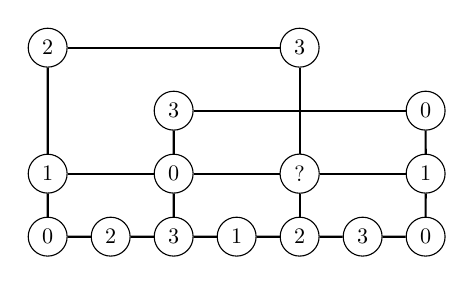
\begin{tikzpicture}[scale=0.8,every node/.style={transform shape}]
			\node[shape=circle,draw=black] (e) at (0,0) {$?$};
			\node[shape=circle,draw=black] (b) at (0,2) {$3$};
			\node[shape=circle,draw=black] (a-1) at (-2,0) {$0$};
			\node[shape=circle,draw=black] (a-2) at (-4,0) {$1$};
			\node[shape=circle,draw=black] (b-1) at (0,-1) {$2$};
			\node[shape=circle,draw=black] (a) at (2,0) {$1$};
			\node[shape=circle,draw=black] (ab) at (2,1) {$0$};
			\node[shape=circle,draw=black] (a-1b) at (-2,1) {$3$};
			\node[shape=circle,draw=black] (a-2b) at (-4,2) {$2$};
			\path[-, thick](ab) edge node[left] {} (a-1b);
			\path[-, thick](a) edge node[left] {} (ab);
			\path[-, thick](a-2b) edge node[left] {} (b);
			\path[-, thick](a-1) edge node[left] {} (a-1b);
			\path[-, thick](a-2) edge node[left] {} (a-2b);
			\path[-, thick](a-1) edge node[left] {} (a-2);
			\path[-, thick](a-1) edge node[left] {} (e);
			\path[-, thick](a) edge node[left] {} (e);
			\path[-, thick](b-1) edge node[left] {} (e);
			\path[-, thick](b) edge node[left] {} (e);
			
			
			\node[shape=circle,draw=black] (b-1a) at (1,-1) {$3$};
			\node[shape=circle,draw=black] (b-1a2) at (2,-1) {$0$};
			\node[shape=circle,draw=black] (b-1a-1) at (-1,-1) {$1$};
			\node[shape=circle,draw=black] (b-1a-2) at (-2,-1) {$3$};
			\node[shape=circle,draw=black] (b-1a-3) at (-3,-1) {$2$};
			\node[shape=circle,draw=black] (b-1a-4) at (-4,-1) {$0$};
			\path[-, thick](b-1) edge node[left] {} (b-1a);
			\path[-, thick](b-1a) edge node[left] {} (b-1a2);
			\path[-, thick](b-1) edge node[left] {} (b-1a-1);
			\path[-, thick](b-1a-1) edge node[left] {} (b-1a-2);
			\path[-, thick](b-1a-2) edge node[left] {} (b-1a-3);
			\path[-, thick](b-1a-3) edge node[left] {} (b-1a-4);
			\path[-, thick](a-2) edge node[left] {} (b-1a-4);
			\path[-, thick](a-1) edge node[left] {} (b-1a-2);
			\path[-, thick](a) edge node[left] {} (b-1a2);
			\end{tikzpicture}
			\caption{Locally admissible pattern for $\mathcal{C}_4$ which cannot be extended to a global configuration.}
			\label{fig:no_extend_gap}
		\end{figure}	
	\end{remark*}
	The previous remark showed a locally admissible pattern that could not be extended to form a valid configuration of the group, and the main property of this example is that although the support of the chosen pattern can be taken to be a connected subgraph of the Cayley graph, it has a ``gap" which allows us to surround a position in such a way that the pattern could not be extended. A way of avoiding these pathological cases is to require the supports of the patterns to have some sort of convexity.
	\begin{lemma} \label{lem:gcs_extend_to_rectangles} For every $n\ge 3$ every $n$-coloring of the rectangle $R_m$ can be extended to a proper $n$-coloring of the rectangle $R_{m+1}$.
	\end{lemma}
	\begin{proof}
		For every $k\in \{0,\ldots,m\}$ we define $$H_k\coloneqq \left(R_{m+1}\backslash R_{m}\right)\cap \{a^ib^k\mid i\ge 0\},$$
		which represents the elements of $R_{m+1}$ of height $k$, outside of the rectangle $R_m$. Note that by definition we have $$R_{m+1}=R_m\cup \bigcup_{k=0}^{m}H_k.$$ Then we can extend the pattern $p$ on $R_m$ by successive colorings (respecting the condition of being a proper coloring) coloring first $H_0$, then $H_1$, and so until we color $H_m$. In each step of this process each vertex has at most $2$ neighbors already colored, so having at least $3$ available colors is enough for this process to be carried out. 
	\end{proof}
	By using the same ideas present in the proof of the previous lemma we obtain the following proposition. Indeed, one can inductively color the rows of the Cayley graph one by one, so that each vertex has at most two colored neighbors at the moment it must choose its color. 
	\begin{proposition}\label{prop:gcs_rectangle_extension} For $n\ge 3$ every locally admissible pattern for $\mathcal{C}_n$ with support a rectangle is globally admissible.
	\end{proposition}

	
	%%%%%%%%%%%%%%%%%%%%%%%%%%%%%%
	
	\subsection{Mixing and frozen colorings}\label{subsection:mixing_and frozen}
Thanks to Proposition \ref{prop:loc_adm_5_colors} we know that for $n\ge 5$ we can extend every admissible pattern to a proper coloring of the Cayley graph of $\BS$, from which we obtain the following mixing property for $\mathcal{C}_n$.
\begin{definition} We say that a subshift $X\subseteq \mathcal{A}^G$ is \textbf{strongly irreducible} if there exists $F\subseteq G$ finite such that for every globally admissible patterns $p,q$ in $X$ with $\mathrm{supp}(p)\cap \mathrm{supp}(q)\cdot F=\varnothing$: $[p]\cap [q]\neq \varnothing$.
\end{definition}

\begin{theorem}\label{thm:gcs_mixing_n5} Let $n\ge 5$ and consider two non-adjacent finite subsets $F_1,F_2\subseteq \BS$, that is, such that 
	$$\left( F_1\cdot \{e_{\BS},a,a^{-1},a,b^{-1}\}\right)\cap F_2=\varnothing.$$
  Then for every choice of (locally) admissible patterns $p_i\in \{0,\ldots,n-1\}^{F_i}, i=1,2,$ there exists $x\in \mathcal{C}_n$ such that $x|_{F_1}=p_1$ and $x|_{F_2}=p_2$. With this we have that for $n\ge 5$ the GCS $\mathcal{C}_n$ is strongly irreducible.
\end{theorem}
\begin{proof}
	The above condition on $F_1$ and $F_2$ means that these two sets are disjoint, and separated by at least one vertex in the Cayley graph of $\BS$. 
	
	Consider two locally admissible patterns $p_i\in \{0,\ldots,n-1\}^{F_i}, i=1,2$. Then we can define a new pattern $p\in \{0,\ldots,n-1\}^{F_1\cup F_2}$ such that $p(f)=p_i(f)$ for $f\in F_i, i=1,2$ consistently, since $F_1\cap F_2=\varnothing.$ This pattern is also locally admissible thanks to the distance existing between $F_1$ and $F_2$, as between every vertex of $F_1$ and every vertex of $F_2$ there is at least one uncolored vertex. Then, according to Proposition \ref{prop:loc_adm_5_colors}, this pattern is globally admissible and hence there exists $x\in \mathcal{C}_n$ such that $x|_{F_1\cup F_2}=p$. This $x$ satisfies $x|_{F_1}=p_1$ and $x|_{F_2}=p_2$ and so we have found the desired point.
\end{proof}


The previous proposition tells us that for $n\ge 5$ the subshift $\mathcal{C}_n$ has a strong mixing property. On the other side, we can see that $\mathcal{C}_2$ has no type of mixing behavior: this $\BS$-subshift is either empty if $N$ is even, or if $N$ is odd then there is no way to assign the same color to two elements of the group $g,h\in \BS$ such that $g^{-1}h\in \left\{a^{2m+1}\mid m\in \mathbb{Z} \right\}$, which forbids the gluing of patterns at arbitrarily large distances. This contrast between $\mathcal{C}_2$ and $\mathcal{C}_n$ for $n\ge 5$ raises the question of what kind of mixing behaviors does $\mathcal{C}_3$ and $\mathcal{C}_4$ have. To study this we will use a similar approach as that of \cite{alon2019mixing}, by introducing the concept of a frozen coloring.
\begin{definition} Let $n\ge 3$. A configuration $x\in \mathcal{C}_n$ is called a \textbf{frozen coloring} if for every $y\in \mathcal{C}_n$ such that there exists a non-empty finite subset $F\subseteq \BS$ with $x|_{F^c}=y|_{F^c}$, then $x= y$. That is, no coloring of $\BS$ other than $x$ can coincide with it outside of a finite set.
\end{definition}

Frozen colorings are configurations in which the neighboring vertices of every finite subset of the Cayley graph determine unequivocally how this subset must be colored, in order to obtain a proper coloring. This behavior is the reason frozen colorings are closely related to the (lack of) mixing properties of the GCS, as the next proposition shows.
\begin{proposition} \label{prop:froz_col_not_si} If $\mathcal{C}_n$ has a frozen coloring, then it is not strongly irreducible.
\end{proposition}
\begin{proof}
	
	Looking for a contradiction, suppose that $\mathcal{C}_n$ is strongly irreducible and $x\in \mathcal{C}_n$ is a frozen coloring. 
	
	Consider any other configuration $y\in \mathcal{C}_n$ such that $y_{e_{\BS}}\neq x_{e_{\BS}}$. As $\mathcal{C}_n$ is strongly irreducible, there exists $F\subseteq G$ finite such that for any two patterns $p,q\in \mathcal{L}(\mathcal{C}_n)$ with $\mathrm{supp}(p)\cap \mathrm{supp}(q)\cdot F=\varnothing$ we have $[p]\cap [q]\neq \varnothing$. Considering the patterns $y|_{e_{\BS}}$ and $x|_{\partial B_M}$, where $\partial B_M\coloneqq \{g\in \BS: |g|=M\}$, for $M$ sufficiently large we have $\partial B_M \cap F= \varnothing$. Then there must exist a coloring $z\in \mathcal{C}_n$ such that $z_{e_{\BS}}=y_{e_{\BS}}\neq x_{e_{\BS}}$, and $z|_{\partial B_M}=x|_{\partial B_M}$. Moreover, we can assume that $z|_{B_{M-1}^c}=x|_{B_{M-1}^c}$, where $B_{M-1}\coloneqq \{g\in \BS: |g|\le M-1 \}$, since $z$ and $x$ coincide on $\partial B_M$ and hence re-coloring $z$ as $x$ outside of this ball gives us a proper coloring. 
	
	With this we have found a configuration $z\in \mathcal{C}_n$ which coincides with $x$ outside of a finite set but is different from $x$ inside it, so we have a contradiction with the fact that $x$ is a frozen coloring. Hence we conclude that a strongly irreducible subshift $\mathcal{C}_n$ cannot have a frozen coloring.
\end{proof}
We already know by Theorem \ref{thm:gcs_mixing_n5} that the GCS $\mathcal{C}_n$ for $n\ge 5$ is strongly irreducible, and hence by the above proposition it cannot have a frozen coloring. On the other hand, as the case $n=3$ is the first non-finite subshift of the GCS's $\mathcal{C}_n$ for $N\ge 2$, it is reasonable to conjecture that its properties must still be somewhat rigid. The next proposition confirms this by showing that $\mathcal{C}_3$ possesses a frozen coloring, and with it exhibits the lack of a strong mixing behavior of the GCS with three colors.
\begin{theorem}\label{thm:existence_frozen_3} The GCS $\mathcal{C}_3\subseteq \{0,1,2\}^{\BS}$ admits a frozen coloring, and hence is not strongly irreducible.
\end{theorem}
\begin{proof}The proof will be divided in three cases, depending on the value of $N \ (\mathrm{mod} \ 3)$. For each one of these cases we will construct explicitly the claimed frozen coloring.
	
	Let us suppose first that $N=1 \ (\mathrm{mod} \ 3)$, and with it for every $i\ge 0$ we have $N^i=1 \ (\mathrm{mod} \ 3)$.
	Let us define the configuration $x\in \{0,1,2\}^{\BS}$ such that for $g=b^{-j}a^k b^i\in \BS$ written in its normal form:
	$$
	x_g\coloneqq 2(i-j)+k \ (\mathrm{mod} \ 3).
	$$
	
	\begin{figure}[H]
		\centering
		\begin{tikzpicture}[scale=0.65,every node/.style={transform shape}]
		\node[font=\Large] at (8,3) {$\vdots$};
		\node[font=\Large] at (4,-1) {$\vdots$};
		\node[font=\Large] at (12,-1) {$\vdots$};
		\node[font=\Large] at (-1,1) {$\cdots$};
		\node[font=\Large] at (17.5,1) {$\cdots$};
		\node[shape=circle,draw=black] (a0) at (0,0) {0};
		\node[shape=circle,draw=black] (a1) at (1,0) {1};
		\node[shape=circle,draw=black] (a2) at (2,0) {2};
		\node[shape=circle,draw=black] (a3) at (3,0) {0};
		\node[shape=circle,draw=black] (a4) at (4,0)  {1};
		\node[shape=circle,draw=black] (a5) at (5,0) {2};
		\node[shape=circle,draw=black] (a6) at (6,0) {0};
		\node[shape=circle,draw=black] (a7) at (7,0) {1};
		\node[shape=circle,draw=black] (a8) at (8,0) {2};
		\node[shape=circle,draw=black] (a9) at (9,0) {0};
		\node[shape=circle,draw=black] (a10) at (10,0) {1};
		\node[shape=circle,draw=black] (a11) at (11,0) {2};
		\node[shape=circle,draw=black] (a12) at (12,0) {0};
		\node[shape=circle,draw=black] (a13) at (13,0) {1};
		\node[shape=circle,draw=black] (a14) at (14,0) {2};
		\node[shape=circle,draw=black] (a15) at (15,0) {0};
		\node[shape=circle,draw=black] (a16) at (16,0) {1};
		\path[-, thick](e) edge node[left] {} (a1);
		\foreach \x[remember=\x as \lastx (initially 0),evaluate=\x as \xx using int(\x)] in {1,...,16}
		{
			\path[-, thick](a\lastx) edge node[left] {} (a\x);
		}
		\node[shape=circle,draw=black] (b) at (0,1) {2};
		\node[shape=circle,draw=black] (a4b) at (4,1) {0};
		\node[shape=circle,draw=black] (a8b) at (8,1) {1};
		\node[shape=circle,draw=black] (a12b) at (12,1) {2};
		\node[shape=circle,draw=black] (a16b) at (16,1) {0};
		\path[-, thick](e) edge node[left] {} (b);
		\path[-, thick](a4) edge node[left] {} (a4b);
		\path[-, thick](a8) edge node[left] {} (a8b);
		\path[-, thick](a12) edge node[left] {} (a12b);
		\path[-, thick](a16) edge node[left] {} (a16b);
		\path[-, thick](b) edge node[left] {} (a4b);
		\path[-, thick](a4b) edge node[left] {} (a8b);
		\path[-, thick](a8b) edge node[left] {} (a12b);
		\path[-, thick](a12b) edge node[left] {} (a16b);
		\node[shape=circle,draw=black] (b2) at (0,2) {1};
		\node[shape=circle,draw=black] (a16b2) at (16,2) {2};
		\path[-, thick](b) edge node[left] {} (b2);
		\path[-, thick](a16b) edge node[left] {} (a16b2);
		\path[-, thick](b2) edge node[left] {} (a16b2);
		\end{tikzpicture}
	\caption{Construction of a frozen $3$-coloring for $N=1\ (\mathrm{mod} \ 3)$.}
	\label{fig:gcs_frozen_3_col_N_1}
	\end{figure}	
	
	Note that $gb=b^{-j}a^k b^{i+1}$ and $ga=b^{-j}a^k b^ia=b^{-j}a^{k+N^i}b^i$. With this, remembering that $N^i =1 \ (\mathrm{mod} \ 3)$ we have
	\begin{align*}
	x_{gb}&=x_g+2 \ (\mathrm{mod} \ 3), \text{ and} \\
	x_{ga}&=x_g+N^i \ (\mathrm{mod} \ 3) =x_g+1 \ (\mathrm{mod} \ 3).
	\end{align*}
	Therefore $x_{gb}\neq x_g$ and $x_{ga}\neq x_g$, and so $x\in \mathcal{C}_3$ defines a proper coloring. Let us see that $x$ defines a frozen coloring: looking for a contradiction let us suppose $y\in \mathcal{C}_3$ is such that there exists a finite subset $F\subseteq \BS$ with $y|_{F^ c}=x|_{F^c}$ and for every $f\in F: \ x_f\neq y_f$. By using the fact that $F$ is finite, and shifting both configurations if necessary, we may assume that $$F\subseteq \{g\in \BS\mid g=a^kb^i, \text{ for some }k\in \mathbb{Z}, i\ge 0\}.$$ 
	Geometrically, this means that $g$ is in the ``upper" section of the Cayley graph of $\BS$, that is, in a sheet having as a base the subgroup $\langle a\rangle$. Now consider $g$ in $F$ which maximizes the value of $i+k$ in its normal form. In other words,
	$$
	g\coloneqq \mathrm{argmax}\{i+k\mid g=a^kb^i\in F, \ k\in \mathbb{Z}, i\ge 0 \}.
	$$
	Then $y_{gb}=x_{gb}=x_g+2\ (\mathrm{mod} \ 3)$, and $y_{ga}=x_{ga}=x_g+1\ (\mathrm{mod} \ 3)$, and so as $y$ defines a proper coloring we must have $y_g=x_g$, but this gives a contradiction since as $g\in F$ we should have $y_g\neq x_g$.
	
	
	Now let us see the case $N=2\ (\mathrm{mod} \ 3)$. Note that now we have that for $i\ge 0$:
	\begin{equation*}	
	N^i=\left\{ 
	\begin{aligned}
	&1 \ (\mathrm{mod} \ 3) \text{ if }i\text{ is even}, \\
	&2 \ (\mathrm{mod} \ 3) \text{ if }i\text{ is odd.} 
	\end{aligned}
	\right.
	\end{equation*}
	Define a configuration  $x\in \{0,1,2\}^{\BS}$ such that for $g=b^{-j}a^k b^i\in \BS$ written in its normal form:
	$$
	x_g\coloneqq i-j+k \ (\mathrm{mod} \ 3).
	$$
	
	
	\begin{figure}[H]
		\centering
		\begin{tikzpicture}[scale=0.65,every node/.style={transform shape}]
		\node[font=\Large] at (8,3) {$\vdots$};
		\node[font=\Large] at (4,-1) {$\vdots$};
		\node[font=\Large] at (12,-1) {$\vdots$};
		\node[font=\Large] at (-1,1) {$\cdots$};
		\node[font=\Large] at (17.5,1) {$\cdots$};
		\node[shape=circle,draw=black] (a0) at (0,0) {0};
		\node[shape=circle,draw=black] (a1) at (1,0) {1};
		\node[shape=circle,draw=black] (a2) at (2,0) {2};
		\node[shape=circle,draw=black] (a3) at (3,0) {0};
		\node[shape=circle,draw=black] (a4) at (4,0)  {1};
		\node[shape=circle,draw=black] (a5) at (5,0) {2};
		\node[shape=circle,draw=black] (a6) at (6,0) {0};
		\node[shape=circle,draw=black] (a7) at (7,0) {1};
		\node[shape=circle,draw=black] (a8) at (8,0) {2};
		\node[shape=circle,draw=black] (a9) at (9,0) {0};
		\node[shape=circle,draw=black] (a10) at (10,0) {1};
		\node[shape=circle,draw=black] (a11) at (11,0) {2};
		\node[shape=circle,draw=black] (a12) at (12,0) {0};
		\node[shape=circle,draw=black] (a13) at (13,0) {1};
		\node[shape=circle,draw=black] (a14) at (14,0) {2};
		\node[shape=circle,draw=black] (a15) at (15,0) {0};
		\node[shape=circle,draw=black] (a16) at (16,0) {1};
		\path[-, thick](e) edge node[left] {} (a1);
		\foreach \x[remember=\x as \lastx (initially 0),evaluate=\x as \xx using int(\x)] in {1,...,16}
		{
			\path[-, thick](a\lastx) edge node[left] {} (a\x);
		}
		\node[shape=circle,draw=black] (b) at (0,1) {1};
		\node[shape=circle,draw=black] (a2b) at (2,1) {0};
		\node[shape=circle,draw=black] (a4b) at (4,1) {2};
		\node[shape=circle,draw=black] (a6b) at (6,1) {1};
		\node[shape=circle,draw=black] (a8b) at (8,1) {0};
		\node[shape=circle,draw=black] (a10b) at (10,1) {2};
		\node[shape=circle,draw=black] (a12b) at (12,1) {1};
		\node[shape=circle,draw=black] (a14b) at (14,1) {0};
		\node[shape=circle,draw=black] (a16b) at (16,1) {2};
		\path[-, thick](e) edge node[left] {} (b);
		\path[-, thick](a2) edge node[left] {} (a2b);
		\path[-, thick](a4) edge node[left] {} (a4b);
		\path[-, thick](a6) edge node[left] {} (a6b);
		\path[-, thick](a8) edge node[left] {} (a8b);
		\path[-, thick](a10) edge node[left] {} (a10b);
		\path[-, thick](a12) edge node[left] {} (a12b);
		\path[-, thick](a14) edge node[left] {} (a14b);
		\path[-, thick](a16) edge node[left] {} (a16b);
		\path[-, thick](b) edge node[left] {} (a2b);
		\path[-, thick](a2b) edge node[left] {} (a4b);
		\path[-, thick](a4b) edge node[left] {} (a6b);
		\path[-, thick](a6b) edge node[left] {} (a8b);
		\path[-, thick](a8b) edge node[left] {} (a10b);
		\path[-, thick](a10b) edge node[left] {} (a12b);
		\path[-, thick](a12b) edge node[left] {} (a14b);
		\path[-, thick](a14b) edge node[left] {} (a16b);
		\node[shape=circle,draw=black] (b2) at (0,2) {2};
		\node[shape=circle,draw=black] (a4b2) at (4,2) {0};		
		\node[shape=circle,draw=black] (a8b2) at (8,2) {1};
		\node[shape=circle,draw=black] (a12b2) at (12,2) {2};
		\node[shape=circle,draw=black] (a16b2) at (16,2) {0};
		\path[-, thick](b) edge node[left] {} (b2);
		\path[-, thick](a4b) edge node[left] {} (a4b2);
		\path[-, thick](a8b) edge node[left] {} (a8b2);
		\path[-, thick](a12b) edge node[left] {} (a12b2);
		\path[-, thick](a16b) edge node[left] {} (a16b2);
		\path[-, thick](b2) edge node[left] {} (a4b2);
		\path[-, thick](a4b2) edge node[left] {} (a8b2);
		\path[-, thick](a8b2) edge node[left] {} (a12b2);
		\path[-, thick](a12b2) edge node[left] {} (a16b2);
		\end{tikzpicture}
	\caption{Construction of a frozen $3$-coloring for $N=2\ (\mathrm{mod} \ 3)$.}
	\label{fig:gcs_frozen_3_col_N_2}
	\end{figure}	
	
	Then as before we have
	\begin{align*}
	x_{gb}&=x_g+1 \ (\mathrm{mod} \ 3), \text{ and} \\
	x_{ga}&=x_g+N^i \ (\mathrm{mod} \ 3),
	\end{align*}
	and so $x_{gb}\neq x_g$ and $x_{ga}\neq x_g$ (since $N^i$ can be either $1$ or $2$). With this we have that $x\in \mathcal{C}_3$ defines a proper coloring, so it only remains to prove that $x$ defines a frozen coloring. Looking for a contradiction, suppose there exists $y\in \mathcal{C}_3$ and a finite set $F\subseteq \BS$ such that $x|_{F^c}=y|_{F^c}$ and for every $f\in F: x_f\neq y_f$. Again, by shifting both configurations if necessary, we may assume that $F\subseteq \{g\in \BS\mid g=a^kb^i, \text{ for some }k\in \mathbb{Z}, i\ge 0\}$. Define $i_{max}\coloneqq \max\{ i\ge 0\mid a^kb^i\in F, \text{ for some }k\in \mathbb{Z}\}$ and $B_{max}\coloneqq\{g=a^kb^i\in F\mid i=i_{max}\}$.
	
	If $i_{max}$ is even, let us take $g=a^kb^i\in B_{max}$ which minimizes the value of $k$. Then as $i_{max}$ is even we have $N^{i_{max}}=1$ and with it $y_{gb}=x_{gb}=x_g+1  \ (\mathrm{mod} \ 3)$, and $y_{ga^{-1}}=x_{ga^{-1}}=x_g-N^{i_{max}} = x_g+2  \ (\mathrm{mod} \ 3)$. But then we must have $y_g=x_g$ and this gives a contradiction since $g\in F$ and therefore $x_g\neq y_g$.
	
	Now if $i_{max}$ is odd, let us consider the element $g=a^kb^i\in B_{max}$ which maximizes the value of $k$. Then as $i_{max}$ is odd we have $N^{i_{max}}=2$ and with it $y_{gb}=x_{gb}=x_g+1  \ (\mathrm{mod} \ 3)$, and $y_{ga}=x_{ga}=x_g+N^{i_{max}} = x_g+2  \ (\mathrm{mod} \ 3)$. But then we must have $y_g=x_g$ and this gives a contradiction since $g\in F$ and therefore $x_g\neq y_g$, proving that $x$ defines a frozen coloring.
	
	
	Finally suppose that $N=0 \ (\mathrm{mod} \ 3)$. The method used on the previous two cases to find a frozen coloring on $\mathcal{C}_3$ was to construct a configuration using a function $f(j,k,i)$ of the coefficients of the normal form of every element of the group, which $\mod \ 3$ had period $3$ on the variable $k$. This cannot be done in the case $N\in 3\mathbb{Z }$ since here the configuration constructed would satisfy $x=\sigma_{a^3}(x)$ and hence $x=\sigma_{a^N}(x)$ (since $N\in 3\mathbb{Z}$). But then by Proposition $\ref{prop:bs_periodicity_p_generalcase}$ the coloring $x$ would have to have monochromatic rows appearing on it, which contradicts the fact that $x\in \mathcal{C}_3$ defines a proper coloring. Nonetheless, using a similar but different kind of function we can define a configuration $x\in \{0,1,2\}^{\BS}$ such that for $g=b^{-j}a^k b^i\in \BS$ written in its normal form:
	$$
	x_g\coloneqq (k \ (\mathrm{mod} \ 2)) + 2(i-j) \ (\mathrm{mod} \ 3).
	$$
	
	\begin{figure}[H]
		\centering
		\begin{tikzpicture}[xscale=0.6,yscale=0.65,every node/.style={transform shape}]
		\node[font=\Large] at (9,3) {$\vdots$};
		\node[font=\Large] at (4,-1) {$\vdots$};
		\node[font=\Large] at (12,-1) {$\vdots$};
		\node[font=\Large] at (-1,1) {$\cdots$};
		\node[font=\Large] at (19.5,1) {$\cdots$};
		\node[shape=circle,draw=black] (e) at (0,0) {0};
		\node[shape=circle,draw=black] (a1) at (1,0) {1};
		\node[shape=circle,draw=black] (a2) at (2,0) {0};
		\node[shape=circle,draw=black] (a3) at (3,0) {1};
		\node[shape=circle,draw=black] (a4) at (4,0)  {0};
		\node[shape=circle,draw=black] (a5) at (5,0) {1};
		\node[shape=circle,draw=black] (a6) at (6,0) {0};
		\node[shape=circle,draw=black] (a7) at (7,0) {1};
		\node[shape=circle,draw=black] (a8) at (8,0) {0};
		\node[shape=circle,draw=black] (a9) at (9,0) {1};
		\node[shape=circle,draw=black] (a10) at (10,0) {0};
		\node[shape=circle,draw=black] (a11) at (11,0) {1};
		\node[shape=circle,draw=black] (a12) at (12,0) {0};
		\node[shape=circle,draw=black] (a13) at (13,0) {1};
		\node[shape=circle,draw=black] (a14) at (14,0) {0};
		\node[shape=circle,draw=black] (a15) at (15,0) {1};
		\node[shape=circle,draw=black] (a16) at (16,0) {0};
		\node[shape=circle,draw=black] (a17) at (17,0) {1};
		\node[shape=circle,draw=black] (a18) at (18,0) {0};
		\path[-, thick](e) edge node[left] {} (a1);
		\foreach \x[remember=\x as \lastx (initially 0),evaluate=\x as \xx using int(\x)] in {1,...,18}
		{
			\path[-, thick](a\lastx) edge node[left] {} (a\x);
		}
		\node[shape=circle,draw=black] (b) at (0,1) {2};
		\node[shape=circle,draw=black] (a3b) at (3,1) {0};
		\node[shape=circle,draw=black] (a6b) at (6,1) {2};
		\node[shape=circle,draw=black] (a9b) at (9,1) {0};
		\node[shape=circle,draw=black] (a12b) at (12,1) {2};
		\node[shape=circle,draw=black] (a15b) at (15,1) {0};
		\node[shape=circle,draw=black] (a18b) at (18,1) {2};
		\path[-, thick](e) edge node[left] {} (b);
		\path[-, thick](a3) edge node[left] {} (a3b);
		\path[-, thick](a6) edge node[left] {} (a6b);
		\path[-, thick](a9) edge node[left] {} (a9b);
		\path[-, thick](a12) edge node[left] {} (a12b);
		\path[-, thick](a15) edge node[left] {} (a15b);
		\path[-, thick](a18) edge node[left] {} (a18b);
		\path[-, thick](b) edge node[left] {} (a3b);
		\path[-, thick](a3b) edge node[left] {} (a6b);
		\path[-, thick](a6b) edge node[left] {} (a9b);
		\path[-, thick](a9b) edge node[left] {} (a12b);
		\path[-, thick](a12b) edge node[left] {} (a15b);
		\path[-, thick](a15b) edge node[left] {} (a18b);
		\node[shape=circle,draw=black] (b2) at (0,2) {1};
		\node[shape=circle,draw=black] (a9b2) at (9,2) {2};
		\node[shape=circle,draw=black] (a18b2) at (18,2) {1};
		\path[-, thick](b) edge node[left] {} (b2);
		\path[-, thick](a9b) edge node[left] {} (a9b2);
		\path[-, thick](a18b) edge node[left] {} (a18b2);
		\path[-, thick](b2) edge node[left] {} (a9b2);
		\path[-, thick](a9b2) edge node[left] {} (a18b2);
		\end{tikzpicture}
	\caption{Construction of a frozen $3$-coloring for $N=0\ (\mathrm{mod} \ 3)$.}
    \label{fig:gcs_frozen_3_col_N_0}
	\end{figure}
	
	
	
	We see that since $N^i$ is odd for every $i\ge 0$ we have:
	\begin{align*}
	x_{gb}&=x_g+2\ (\mathrm{mod} \ 3), \text{ and} \\
	x_{ga}&=(k+N^i \ (\mathrm{mod} \ 2)) + 2(i-j) \ (\mathrm{mod} \ 3)=x_g+1 \ (\mathrm{mod} \ 3),
	\end{align*}
	from which $x\in \mathcal{C}_3$ defines a proper coloring, and we can proceed as we did previously in the case $N^i=1\ (\mathrm{mod} \ 3)$. That is, to prove that $x$ defines a frozen coloring we suppose $y\in \mathcal{C}_3$ is such that there exists a finite subset $F\subseteq \BS$ with $y|_{F^ c}=x|_{F^c}$ and for every $f\in F: \ x_f\neq y_f$. By shifting both configurations if necessary, we may assume that $F\subseteq \{g\in \BS\mid g=a^kb^i, \text{ for some }k\in \mathbb{Z}, i\ge 0\}$. Now let us consider $g$ in $F$ which maximizes the value of $i+k$ in its normal form. Then $y_{gb}=x_{gb}=x_g+2\ (\mathrm{mod} \ 3)$, and $y_{ga}=x_{ga}=x_g+1\ (\mathrm{mod} \ 3)$, and so as $y$ defines a proper coloring we must have $y_g=x_g$, but this gives a contradiction since as $g\in F$ we should have $y_g\neq x_g$. Hence we see that $x$ a frozen coloring.
	
	To finish the proof we simply use the previous proposition to see that $\mathcal{C}_3$ cannot be strongly irreducible, as we have constructed a frozen coloring in it.
\end{proof}

This last theorem together with the previous comments settle the existence of frozen colorings for $n=3$ and $n\ge 5$. To tackle the case of four colors, and in the process give an alternative proof of the lack of frozen colorings for $n\ge 5$, we will use a proposition from \cite{alon2019mixing} used in that paper to prove the lack of frozen $n$-colorings in $\mathbb{Z}^d$ for $n\ge d+2$.

\begin{proposition}[{\cite[Proposition~2.2]{alon2019mixing}}]\label{prop:nofroz_graph} For a graph $\Gamma$ let us define its \textbf{edge-isoperimetric constant} by
	$$
	i_e(\Gamma)\coloneqq \inf_{F\subseteq \Gamma \text{ finite}}\frac{|E(F,\Gamma\backslash F)|}{|F|},
	$$
	where $E(F,\Gamma\backslash F)$ are the edges of $\Gamma$ connecting vertices from $F$ to $\Gamma\backslash F$. Denote by $\Delta$ the maximum degree of $\Gamma$. Then for every $n>\frac{1}{2}\Delta+\frac{1}{2}i_e(\Gamma)+1$ there do not exist frozen $n$-colorings of $\Gamma$.
\end{proposition}
\begin{theorem}\label{thm:no_frozen_n_ge_4} For $n\ge 4$ the GCS $\mathcal{C}_n$ does not admit a frozen coloring.
\end{theorem}
\begin{proof}
	Denoting by $\Gamma$ the Cayley graph of $\BS$ its maximum degree is $\Delta=4$, and if we prove that $i_e(\Gamma)=0$ we will have that, using proposition \ref{prop:nofroz_graph}, for $n>\frac{1}{2}\cdot 4+\frac{1}{2}\cdot 0+1=3$ this graph does not admit frozen $n$-colorings, proving the statement.
	
	Let us see that $i_e(\Gamma)=0$. Consider for every $k\ge 1: \ \gamma_{k}\coloneqq E(R_k,\Gamma\backslash R_k)$. We see that $\gamma_1=2N+2$, and that for every $k\ge 2$:
	$$
	\gamma_k=N^k+2+N(\gamma_{k-1}-N^{k-1})=2+N\gamma_{k-1},
	$$
	by using the fact that the $N$ sheets arising from the base of the rectangle $R_k$ are copies of the rectangle $R_{k-1}$. 
	With this we have that 
	$$
	\gamma_{k+1}-\gamma_{k}=N(\gamma_k-\gamma_{k-1}), \ \gamma_{2}-\gamma_{1}=2N^2,
	$$
	and so $\gamma_{k}-\gamma_{k-1}=2N^k$, for every $k\ge 2$. Now summing this equality from $k=2$ to $k=m$ we see that
	\begin{align*}
	\gamma_{m}-(2N+2)=\gamma_{m}-\gamma_{1}=\sum_{k=2}^m \gamma_{k}-\gamma_{k-1}&=2\sum_{k=2}^m N^k \\
	&= 2\frac{N^{m+1}-N^2}{N-1},
	\end{align*}
	and hence $\gamma_{m}=2\frac{N^{m+1}-1}{N-1}$. From this calculation we can estimate the edge-isoperimetric constant:
	$$
	i_e(\Gamma)\le \liminf_{m\to \infty}\frac{|E(R_m,\Gamma\backslash R_m|)}{|R_m|}=\liminf_{m\to \infty}\frac{\gamma_m}{|R_m|}=\liminf_{m\to \infty}\frac{2}{mN^m}\frac{N^{m+1}-1}{N-1}=0,
	$$
	and so $i_e(\Gamma)=0$ as we had claimed at the beginning of the proof.
\end{proof}
	
	%%%%%%%%%%%%%%%%%%%%%%%%%%%%%%
	
\subsection{Topological entropy}
We finish this section by focusing our attention to the topological entropy of the GCS $\mathcal{C}_n$. By estimating in how many different ways a pattern defined on a rectangle can be extended to a bigger one, we obtain the following bounds.
\begin{theorem}\label{thm:gcs_entropy_estimates} For $n\ge 3$, we have the following estimate for the topological entropy of the GCS $\mathcal{C}_n$:
	$$
	\log(n-2)\le \htop(\mathcal{C}_n)\le \log(n-1).
	$$
\end{theorem}
\begin{proof}
	Let us see that $\htop(\mathcal{C}_n)\le \log(n-1)$: a coloring of the rectangle $R_m$ may be extended to a coloring of the rectangle $R_{m+1}$ by coloring the remaining vertices having on each one at most $n-1$ options. With this
	\begin{align*}
	|\mathcal{L}_{R_{m+1}}(\mathcal{C}_n)|\le |\mathcal{L}_{R_m}(\mathcal{C}_{n})|(n-1)^{|R_{m+1}\backslash R_m|}.
	\end{align*}
	A simple calculation shows that $|R_{m+1}\backslash R_{m}|=N^m(mN+N-m)$. 
	With this:
	\begin{align*}
	\frac{1}{|R_{m+1}|}\log|\mathcal{L}_{R_{m+1}}(\mathcal{C}_n)|&=\frac{1}{(m+1)N^{m+1}}\log|\mathcal{L}_{R_{m+1}}(\mathcal{C}_n)|\\
	&\le \frac{1}{(m+1)N^{m+1}}\log|\mathcal{L}_{R_m}(\mathcal{C}_{n})|+\frac{N^m(mN+N-m)}{(m+1)N^{m+1}}\log(n-1)\\
	&=\frac{1}{N}\frac{m}{m+1}\frac{1}{mN^{m}}\log|\mathcal{L}_{R_m}(\mathcal{C}_{n})|+ \frac{mN+N-m}{m+1}\frac{1}{N}\log(n-1)\\
	&=\frac{1}{N}\frac{m}{m+1}\frac{1}{|R_m|}\log|\mathcal{L}_{R_m}(\mathcal{C}_{n})|+ \frac{m(N-1)+N}{m+1}\frac{1}{N}\log(n-1).
	\end{align*}
	Taking the limit $m\to \infty$ we arrive at
	\begin{align*}
	\htop(\mathcal{C}_n)&=\lim_{m\to \infty }	\frac{1}{|R_{m+1}|}\log|\mathcal{L}_{R_{m+1}}(\mathcal{C}_n)|\\
	&\le \lim_{m\to \infty }\frac{1}{N}\frac{m}{m+1}\frac{1}{|R_m|}\log|\mathcal{L}_{R_m}(\mathcal{C}_{n})| +\lim_{m\to \infty }\frac{m(N-1)+N}{m+1}\frac{1}{N}\log(n-1)\\
	&= \frac{1}{N}\htop(\mathcal{C}_n)+\frac{N-1}{N}\log(n-1),
	\end{align*}
	from where 
	$$\htop(\mathcal{C}_n)\le \log(n-1).$$
	
	
	Now let us see that $\htop(\mathcal{C}_n)\ge \log(n-2)$:
	the rectangle $R_m$ can be colored starting from the upper levels to the lower levels, ensuring at least $n-2$ color options at each element, since in this way each vertex of the Cayley graph has at most two neighbors already colored. Then this coloring can be extended to the whole graph by using Proposition \ref{prop:gcs_rectangle_extension} and hence forming a globally admissible configuration for $\mathcal{C}_n$. From this we arrive at
	\begin{align*}
	|\mathcal{L}_{R_m}(\mathcal{C}_{n})|\ge (n-2)^{|R_m|},
	\end{align*}
	and so $\htop(\mathcal{C}_n)\ge \log(n-2)$.
\end{proof}
In particular, the lower bound from the previous proposition shows us that $\htop(\mathcal{C}_n)>0$ for every $n\ge 4$, but gives us no new information for the case of three colors $\mathcal{C}_3$, since by definition $\htop(\mathcal{C}_3)\ge 0$. In the next proposition we show that indeed $\htop(\mathcal{C}_3)>0$, dividing the proof in two cases depending on the parity of $N$. If $N$ is odd we can exploit the fact that the Cayley graph of $\BS$ is bipartite (we know this since we have already constructed a $2$-coloring of it in Proposition \ref{prop:GCS_nonemptiness}, or equivalently observing that it has no odd cycles) to give a straightforward proof, while in the case of even $N$ we give a more delicate construction to arrive at the same result.
\begin{theorem}\label{thm:C_3_has_positive_entropy} The GCS $\mathcal{C}_3\subseteq \{0,1,2\}^{\BS}$ has positive topological entropy.
\end{theorem}
\begin{proof}
	Let us start with the case of odd $N$. Here the Cayley graph of $\BS$ is bipartite and hence so is every rectangle $R_m$, for $m\ge 1$. Consider a \textit{partition} of $R_m$ into two sets $A$ and $B$, meaning that all edges of the graph are composed of a vertex in $A$ and a vertex in $B$. Then one of them, which we take to be $A$ without loss of generality, must have cardinality at least $\frac{1}{2}|R_m|$. Then we can create proper colorings of $R_m$ by coloring the vertices of $B$ with one color and have the freedom to choose between two colors for every vertex of $A$, and then extend this pattern on $R_m$ to the rest of the group as was said earlier.
	
	With the above we can estimate a lower bound for the number of proper colorings of $R_m$ by
	$$
	|\mathcal{L}_{R_m}(\mathcal{C}_3)|\ge 2^{|A|}\ge 2^{\frac{1}{2}|R_m|}.
	$$
	Then taking logarithm and dividing by $|R_m|$ we arrive at
	$$
	\frac{1}{|R_m|}\log |\mathcal{L}_{R_m}(\mathcal{C}_3)| \ge \frac{1}{2}\log (2),
	$$
	to finally take limit as $m\to \infty$ and obtain
	$$
	\htop(\mathcal{C}_3)\ge \frac{1}{2}\log(2)>0,
	$$
	which is what we wanted.
	
	
	Now consider the case of even $N$. For $m\ge 1$ we define a pattern $p\in \mathcal{A}^{R_{2m}}$, where some of the vertices of this rectangle will have the freedom of being assigned the symbol $1$ or $2$, in either case remaining a proper $3$-coloring of $R_{2m}$.
	
	First let us define 
	$$
	p|_{[e_{\BS},a^{N^{2m}-1}]}=\left(0(12)^{2N}\right)^{\infty}|_{[0,N^{2m}-1]},
	$$
	and for $i\in \{0,\ldots, N^{2m}-1 \}$, $j\in \{0,\ldots, m-1 \}$ define
	$$
	p_{a^{i}b^{2j}}=p_{a^i}.
	$$
	That is, the symbols we see in the $a$-rows at even level of $R_{2m}$ are copies of the sequence found in the base of the rectangle. Now we proceed to define the pattern $p$ at the $a$-rows of odd level. Define for $i\in \left\{0,\ldots, \left\lfloor \frac{N^{2m}}{2N+1}\right\rfloor-1  \right\}$, $k\in \{0,\ldots,2N\}$, $j\in \{0,\ldots,m-1\}$ and any choice of $\alpha_{i,j,k}\in \{0,1\}$:
	\begin{equation*}
	p_{a^{(2N+1)i+k}b^{2j+1}}=\left\{
	\begin{aligned}
	&\alpha_{i,j,k} \text{ if }k=0,\\
	& 0\text{ if }k=N \text{ or }k=N+1,\\
	& 2\text{ if }k\text{ is even and }k\neq N,\\
	& 1\text{ if }k\text{ is odd and }k\neq N+1.\\
	\end{aligned}
	\right.
	\end{equation*}
	With the above we are assigning to each $a$-row at odd level of $R_m$ (a subword of) the sequence $\left(\alpha_{i,j,k}\ 0\ (12)^{2N-2}\right)^{\infty}$, where every choice of $\alpha(i,j,k)\in \{1,2\}$ gives rise to a different pattern.
	
		\begin{figure}[H]
		\centering
		\begin{tikzpicture}[scale=0.6,every node/.style={transform shape}]
		\node[font=\Large] at (8,3) {$\vdots$};
		\node[font=\Large] at (4,-1) {$\vdots$};
		\node[font=\Large] at (12,-1) {$\vdots$};
		\node[font=\Large] at (-1,1) {$\cdots$};
		\node[font=\Large] at (17.5,1) {$\cdots$};
		\node[shape=circle,draw=black] (a0) at (0,0) {0};
		\node[shape=circle,draw=black] (a1) at (1,0) {1};
		\node[shape=circle,draw=black] (a2) at (2,0) {2};
		\node[shape=circle,draw=black] (a3) at (3,0) {1};
		\node[shape=circle,draw=black] (a4) at (4,0)  {2};
		\node[shape=circle,draw=black] (a5) at (5,0) {0};
		\node[shape=circle,draw=black] (a6) at (6,0) {1};
		\node[shape=circle,draw=black] (a7) at (7,0) {2};
		\node[shape=circle,draw=black] (a8) at (8,0) {1};
		\node[shape=circle,draw=black] (a9) at (9,0) {2};
		\node[shape=circle,draw=black] (a10) at (10,0) {0};
		\node[shape=circle,draw=black] (a11) at (11,0) {1};
		\node[shape=circle,draw=black] (a12) at (12,0) {2};
		\node[shape=circle,draw=black] (a13) at (13,0) {1};
		\node[shape=circle,draw=black] (a14) at (14,0) {2};
		\node[shape=circle,draw=black] (a15) at (15,0) {0};
		\node[shape=circle,draw=black] (a16) at (16,0) {1};
		\path[-, thick](e) edge node[left] {} (a1);
		\foreach \x[remember=\x as \lastx (initially 0),evaluate=\x as \xx using int(\x)] in {1,...,16}
		{
			\path[-, thick](a\lastx) edge node[left] {} (a\x);
		}
		\node[shape=circle,draw=black] (b) at (0,1) {?};
		\node[shape=circle,draw=black] (a2b) at (2,1) {0};
		\node[shape=circle,draw=black] (a4b) at (4,1) {2};
		\node[shape=circle,draw=black] (a6b) at (6,1) {1};
		\node[shape=circle,draw=black] (a8b) at (8,1) {0};
		\node[shape=circle,draw=black] (a10b) at (10,1) {?};
		\node[shape=circle,draw=black] (a12b) at (12,1) {0};
		\node[shape=circle,draw=black] (a14b) at (14,1) {2};
		\node[shape=circle,draw=black] (a16b) at (16,1) {1};
		\path[-, thick](e) edge node[left] {} (b);
		\path[-, thick](a2) edge node[left] {} (a2b);
		\path[-, thick](a4) edge node[left] {} (a4b);
		\path[-, thick](a6) edge node[left] {} (a6b);
		\path[-, thick](a8) edge node[left] {} (a8b);
		\path[-, thick](a10) edge node[left] {} (a10b);
		\path[-, thick](a12) edge node[left] {} (a12b);
		\path[-, thick](a14) edge node[left] {} (a14b);
		\path[-, thick](a16) edge node[left] {} (a16b);
		\path[-, thick](b) edge node[left] {} (a2b);
		\path[-, thick](a2b) edge node[left] {} (a4b);
		\path[-, thick](a4b) edge node[left] {} (a6b);
		\path[-, thick](a6b) edge node[left] {} (a8b);
		\path[-, thick](a8b) edge node[left] {} (a10b);
		\path[-, thick](a10b) edge node[left] {} (a12b);
		\path[-, thick](a12b) edge node[left] {} (a14b);
		\path[-, thick](a14b) edge node[left] {} (a16b);
		\node[shape=circle,draw=black] (b2) at (0,2) {0};
		\node[shape=circle,draw=black] (a4b2) at (4,2) {2};		
		\node[shape=circle,draw=black] (a8b2) at (8,2) {1};
		\node[shape=circle,draw=black] (a12b2) at (12,2) {2};
		\node[shape=circle,draw=black] (a16b2) at (16,2) {1};
		\path[-, thick](b) edge node[left] {} (b2);
		\path[-, thick](a4b) edge node[left] {} (a4b2);
		\path[-, thick](a8b) edge node[left] {} (a8b2);
		\path[-, thick](a12b) edge node[left] {} (a12b2);
		\path[-, thick](a16b) edge node[left] {} (a16b2);
		\path[-, thick](b2) edge node[left] {} (a4b2);
		\path[-, thick](a4b2) edge node[left] {} (a8b2);
		\path[-, thick](a8b2) edge node[left] {} (a12b2);
		\path[-, thick](a12b2) edge node[left] {} (a16b2);
		\end{tikzpicture}
		\caption{Nodes with a ``?'' have freedom of choosing between a symbol ``1'' or ``2'', since all their neighbours have ``0''s in them.}
	\end{figure}
	
	The above shows that
	$$
	|\mathcal{L}_{R_{2m}}(\mathcal{C}_3)|\ge 2^{m\left\lfloor \frac{N^{2m}}{2N+1}\right\rfloor },
	$$
	and hence
	\begin{align*}
	\frac{1}{|R_{2m}|}\log |\mathcal{L}_{R_{2m}}(\mathcal{C}_3)|&\ge\frac{m\left\lfloor \frac{N^{2m}}{2N+1}\right\rfloor}{2mN^{2m}}\log(2) \\
	&\ge \frac{\frac{N^{2m}}{2N+1}-1}{2N^{2m}}\log(2).
	\end{align*}
	Finally, taking limit as $m\to\infty$ we obtain
	$$
	\htop(\mathcal{C}_3)\ge \frac{1}{2(2N+1)}\log(2)>0.
	$$
\end{proof}	
%%%%%%%%%%%%%%%%%%%%%%%%%%%%%%
%%%%%%%%%%%%%%%%%%%%%%%%%%%%%%

\section{Possible generalizations}
		The behavior of configurations in $\BS$-subshifts found in the results of this paper seems to actually arise from more fundamental results, in a slighter abstract context.
		
		We say that an HNN-extension $G*_{\psi}$ is \textbf{ascending} if one of the associated subgroups being conjugated is $G$ itself, that is, considering $\psi:G\to G$ to be an injective homomorphism. All properties for $\BS$ mentioned in Section \ref{section:preliminaries} generalize to ascending HNN-extensions $G*_{\psi}$, for $G$ an abelian finitely generated group. In particular, we can find an analogous normal form to that of Proposition \ref{prop:normalform_bsgroups} changing $N\mathbb{Z}$ for $\psi(G)$, and a F\o lner sequence similar to the rectangles of Proposition \ref{prop:rectangles_and_folner}.
		
		Fixing a generating set for $G$, the Cayley graph of an ascending HNN-extension $G*_{\psi}$ of an abelian finitely generated group resembles the one described at the end of Section \ref{section:preliminaries} for $\BS$. It is composed of copies of the Cayley graph of $G$ connected through the generator $t$, in such a way that each one has above it $|G:\psi(G)|$ copies of itself. Making an analogous between $a$-rows in the Cayley graph of $\BS$ and copies of $G$ in the Cayley graph of $G*_{\psi}$ we obtain the following generalization of Theorem \ref{thm:summary_weak_periodicity}.
	
	\begin{theorem}
		Consider $\mathcal{A}$ a finite alphabet, $G$ an abelian finitely generated group, $G*_{\psi}$ an ascending HNN-extension and $x\in \mathcal{A}^{G*_{\psi}}$. Suppose we find a subgroup $H\le G$ with $\psi(H)\subseteq H$ such that there exists an $\ell\ge 0$ with $\psi^\ell(H)\le \mathrm{Stab}(x)$. Then all copies of $G$ of level higher than $\ell$ must be $H$-periodic.
		
		If $X$ is a $G*_{\psi}$-subshift containing a configuration as above, then it must also contain one in which every copy of $G$ is $H$-periodic, which can be chosen to be strongly periodic if we further assume that $X$ is an SFT and $H=G$. 
	\end{theorem}

	
It is also interesting to think about how the properties from Section \ref{section:graph_coloring_subshifts} for graph-coloring subshifts in $\BS$ generalize to this more fundamental context. The answers will now probably be separated in two cases depending on the nature of the group $G$, with respect to whether it is bipartite or not. Results will also probably depend on the value of $|G:\psi(G)|$, since this number will play a role in the length of the new cycles that arise in the Cayley graph of $G*_{\psi}$, in contrast with those found in $G$.

The method used to find the topological entropy bounds for GCS in $\BS$ was counting patterns using rectangles, and thus should be able to be replicated to some extent for $G*_{\psi}$, using natural generalizations of rectangles to this group. 
	\begin{question*}
How do the topological entropy related results from Theorem \ref{thm:summary_gcs_entropy} generalize to GCS in $G*_{\psi}$?
\end{question*}
With respect to frozen colorings, Proposition \ref{prop:nofroz_graph} was fundamental in our study of said configurations, and it will probably be too when studying them in $G*_{\psi}$. A first approach when computing the edge-isoperimetric constant of the Cayley graph $\Gamma$ of $G*_{\psi}$ should be to determine the value of $E(R_k,\Gamma\backslash R_k)$, for $R_k$ the generalization of rectangles to this group, as we did in the proof of Proposition \ref{thm:no_frozen_n_ge_4}.
\begin{question*}
	For which $n$ does $G*_{\psi}$ admit frozen $n$-colorings?
\end{question*}
	
	\textbf{Acknowledgements}. I would like to thank my Master's advisor Michael Schraudner for his continuous support, and Nathalie Aubrun for her helpful comments and ideas. This work was developed as part of a Master's degree thesis, partially supported by CONICYT-PFCHA/Mag\'ister Nacional/2019 - 22190176.
	
	%%%%%%%%%%%%%%%%%%%%%%%
	%%%%%%%%%%%%%%%%%%%%%%%
	\bibliographystyle{plain}
	\bibliography{bibliography}{}
\end{document}